\setstretch{1}
\setlength{\parskip}{\baselineskip}

\section{Introduction}
The Netlist Reader subsystem serves as the front-end input ingestion and compilation module for the circuit simulator. Its primary responsibility is the transformation of hierarchical SPICE circuit netlists into structured, memory-mapped data structures through lexical normalization, macro subcircuit expansion, dynamic parameter evaluation, and semantic verification prior to downstream simulation setup.

Rather than populating numerical solver matrices directly, the Netlist Reader operates as a decoupled data provider. Upon completing its compilation pipeline, it exposes resolved structural entities—specifically the node mapping index, technology model database, and flattened component vectors—to the downstream \texttt{MathematicalModelling} subsystem, which physically realizes the devices and populates the Modified Nodal Analysis (MNA) matrices. Concurrently, simulation commands and control options are exposed to the core \texttt{Simulator} engine, enabling it to select appropriate device stamping modes and execute solver algorithms. To guarantee simulation determinism across execution runs, the subsystem executes a mandatory state isolation protocol before processing a netlist deck, resetting internal symbol tables, model registries, and expression evaluation caches.


\section{Supported SPICE Syntax and Conventions}
\label{sec:supported_syntax}

This section serves as a reference manual for the SPICE syntax and netlist conventions supported by the simulator. The subsections below outline the valid structural statements, physical component declarations, semiconductor model cards, numerical options, analysis directives, and control scripting features handled by the reader.

\subsection{Lexical Conventions and Mathematical Expressions}

\subsubsection{Circuit Title Line}
\begin{compactitem}
    \item \textbf{Syntax:} \\
    \texttt{<title\_text>} (First non-comment physical line)
    \item \textbf{Rules:} The very first non-comment line of a netlist file is automatically defined as the circuit title. Any text on this line is treated as design metadata and is not evaluated as an operational circuit statement.
\end{compactitem}

\subsubsection{End of Deck Directive (\texttt{.end})}
\begin{compactitem}
    \item \textbf{Syntax:} \\
    \texttt{.end}
    \item \textbf{Rules:} Marks the absolute termination of the circuit netlist deck. All text and statements appearing below the \texttt{.end} directive are ignored during simulation setup.
\end{compactitem}

\subsubsection{Comment Lines and Inline Comments}
\begin{compactitem}
    \item \textbf{Syntax:} \\
    \texttt{* comment}, \texttt{\# comment}, \texttt{; comment}, or \texttt{// comment}
    \item \textbf{Rules:} Lines beginning with \texttt{*}, \texttt{\#}, \texttt{;}, or \texttt{//} are treated as full-line comments. Inline comments are supported using \texttt{;}, \texttt{\#}, or \texttt{//}. All comments are stripped prior to statement analysis.
\end{compactitem}

\subsubsection{Line Continuation Character (\texttt{+})}
\begin{compactitem}
    \item \textbf{Syntax:} \\
    \texttt{+ continuation\_tokens}
    \item \textbf{Rules:} A plus sign (\texttt{+}) placed as the first non-whitespace character of a physical line joins that line directly to the end of the preceding logical statement, allowing long declarations to be formatted across multiple physical lines.
\end{compactitem}

\subsubsection{Engineering Scale Multipliers and Numeric Literals}
\begin{compactitem}
    \item \textbf{Syntax:} \\
    \texttt{value[multiplier][unit]} (e.g., \texttt{10k}, \texttt{2.5uF}, \texttt{1MEG})
    \item \textbf{Rules:} Numeric values support standard case-insensitive engineering scale multipliers. Recognized suffixes include \texttt{t} ($10^{12}$), \texttt{g} ($10^9$), \texttt{meg} ($10^6$), \texttt{k} ($10^3$), \texttt{m} ($10^{-3}$), \texttt{u} or UTF-8 \(\mu\) ($10^{-6}$), \texttt{n} ($10^{-9}$), \texttt{p} ($10^{-12}$), and \texttt{f} ($10^{-15}$). Trailing physical units (such as \texttt{Hz}, \texttt{F}, \texttt{V}, or \texttt{A}) are automatically ignored.
\end{compactitem}

\subsubsection{Brace-Enclosed Mathematical Expressions}
\begin{compactitem}
    \item \textbf{Syntax:} \\
    \texttt{\{expression\}} (e.g., \texttt{\{(vcc * 0.5) / 10k\}})
    \item \textbf{Rules:} Mathematical expressions enclosed in curly braces support standard arithmetic operators (\texttt{+}, \texttt{-}, \texttt{*}, \texttt{/}), unary sign operations, grouping parentheses \texttt{()}, and active parameter identifiers. Nested curly braces (e.g., \texttt{\{a+\{b\}\}}) are not supported.
\end{compactitem}

\subsection{Physical Components and Waveforms}

Device statements are routed based on their single-character leading prefix. Positional arguments and optional key-value parameter pairs are validated for twelve distinct device classes:

\begin{table}[H]
\centering
\small
\begin{tabular}{|c|l|p{4.2cm}|p{4.5cm}|}
\hline
\textbf{Prefix} & \textbf{Device Category} & \textbf{SPICE Syntax Format} & \textbf{Validation Constraints \& Options} \\
\hline
\texttt{R} & Resistor & \texttt{Rname n1 n2 value} & Requires 4 positional tokens. \\
\hline
\texttt{C} & Capacitor & \texttt{Cname n1 n2 value} & Requires 4 positional tokens. \\
\hline
\texttt{L} & Inductor & \texttt{Lname n1 n2 value} & Requires 4 positional tokens. \\
\hline
\texttt{V} / \texttt{I} & Independent Source & \texttt{Vname n+ n- [dc] [ac ...] [func]} & DC/AC specs; transient functions. \\
\hline
\texttt{E} & VCVS & \texttt{Ename n+ n- ns+ ns- gain} & Requires 6 tokens (voltage gain). \\
\hline
\texttt{G} & VCCS & \texttt{Gname n+ n- ns+ ns- transcond} & Requires 6 tokens (transconductance). \\
\hline
\texttt{F} & CCCS & \texttt{Fname n+ n- vcontrol gain} & Requires 5 tokens (current gain). \\
\hline
\texttt{H} & CCVS & \texttt{Hname n+ n- vcontrol transres} & Requires 5 tokens (transresistance). \\
\hline
\texttt{D} & Diode & \texttt{Dname n1 n2 model [options]} & Options: \texttt{area}, \texttt{t}/\texttt{temp}, \texttt{off}. \\
\hline
\texttt{M} & MOSFET & \texttt{Mname nd ng ns nb model [options]} & Options: \texttt{w}, \texttt{l} ($w>0, l>0$ strictly). \\
\hline
\texttt{Q} & BJT & \texttt{Qname nc nb ne [ns] [tj] model [opts]} & 4--6 positional tokens; \texttt{area}, \texttt{m}, \texttt{off}. \\
\hline
\texttt{J} & JFET & \texttt{Jname nd ng ns model [area] [opts]} & Options: \texttt{area}, \texttt{temp}, \texttt{off}. \\
\hline
\end{tabular}
\caption{Complete physical component syntax specifications}
\label{tab:component_syntax_complete}
\end{table}

\subsubsection{Resistors (\texttt{R})}
\begin{compactitem}
    \item \textbf{Syntax:} \\
    \texttt{Rname n1 n2 value}
    \item \textbf{Rules:} Requires exactly four positional arguments representing the component name, positive node, negative node, and nominal resistance value.
\end{compactitem}

\subsubsection{Capacitors (\texttt{C}) \& Inductors (\texttt{L})}
\begin{compactitem}
    \item \textbf{Syntax:} \\
    \texttt{Cname n1 n2 value} or \texttt{Lname n1 n2 value}
    \item \textbf{Rules:} Requires exactly four positional arguments representing the component name, positive node, negative node, and nominal capacitance or inductance value.
\end{compactitem}

\subsubsection{Independent Sources (\texttt{V}, \texttt{I})}
\begin{compactitem}
    \item \textbf{Syntax:} \\
    \texttt{Vname n+ n- [dc\_val] [ac [mag [phase]]] [trans\_func]} or \texttt{Iname n+ n- [dc\_val] [ac [mag [phase]]] [trans\_func]}
    \item \textbf{Rules:} Specifies independent voltage or current sources connected between positive and negative terminals. Operating values may be set for DC analysis (defaulting to $0.0$), small-signal AC analysis (defaulting to magnitude $1.0$ and phase $0.0$), or transient analysis using dynamic waveform functions.
\end{compactitem}

\subsubsection{Sinusoidal Transient Waveform (\texttt{sin})}
\begin{compactitem}
    \item \textbf{Syntax:} \\
    \texttt{sin(vo va freq [td] [theta] [phase])}
    \item \textbf{Rules:} Generates a continuous sinusoidal waveform defined by DC offset (\texttt{vo}), amplitude (\texttt{va}), frequency (\texttt{freq}), delay time (\texttt{td}), damping factor (\texttt{theta}), and phase offset (\texttt{phase}).
\end{compactitem}

\subsubsection{Pulse Transient Waveform (\texttt{pulse})}
\begin{compactitem}
    \item \textbf{Syntax:} \\
    \texttt{pulse(v1 v2 [td] [tr] [tf] [pw] [per] [np])}
    \item \textbf{Rules:} Generates a periodic pulse train specified by initial level (\texttt{v1}), pulsed level (\texttt{v2}), delay time (\texttt{td}), rise time (\texttt{tr}), fall time (\texttt{tf}), pulse width (\texttt{pw}), period (\texttt{per}), and pulse count (\texttt{np}).
\end{compactitem}

\subsubsection{Exponential Transient Waveform (\texttt{exp})}
\begin{compactitem}
    \item \textbf{Syntax:} \\
    \texttt{exp(v1 v2 [td1] [tau1] [td2] [tau2])}
    \item \textbf{Rules:} Generates a dual exponential transient defined by initial level (\texttt{v1}), pulsed level (\texttt{v2}), rise delay (\texttt{td1}), rise time constant (\texttt{tau1}), decay delay (\texttt{td2}), and decay time constant (\texttt{tau2}).
\end{compactitem}

\subsubsection{Piecewise Linear Transient Waveform (\texttt{pwl})}
\begin{compactitem}
    \item \textbf{Syntax:} \\
    \texttt{pwl(t1 v1 t2 v2 ...)}
    \item \textbf{Rules:} Constructs an arbitrary piecewise linear waveform defined by sequential time-voltage coordinate pairs. Requires an even number of arguments.
\end{compactitem}

\subsubsection{Voltage-Controlled Sources (\texttt{E}, \texttt{G})}
\begin{compactitem}
    \item \textbf{Syntax (VCVS / VCCS):} \\
    \texttt{Ename n+ n- ns+ ns- value} or \texttt{Gname n+ n- ns+ ns- value}
    \item \textbf{Rules:} Requires six positional arguments mapping output terminal nodes, controlling terminal nodes, and a constant voltage gain ($E$) or transconductance factor ($G$).
\end{compactitem}

\subsubsection{Current-Controlled Sources (\texttt{F}, \texttt{H})}
\begin{compactitem}
    \item \textbf{Syntax (CCCS / CCVS):} \\
    \texttt{Fname n+ n- vsource value} or \texttt{Hname n+ n- vsource value}
    \item \textbf{Rules:} Requires five positional arguments mapping output terminal nodes, controlling independent voltage source name (\texttt{vsource}), and a constant current gain ($F$) or transresistance factor ($H$).
\end{compactitem}

\subsubsection{Diodes (\texttt{D})}
\begin{compactitem}
    \item \textbf{Syntax:} \\
    \texttt{Dname n1 n2 model\_id [area=val] [t=val] [temp=val] [off]}
    \item \textbf{Rules:} Specifies a junction diode referencing a valid device model card. Optional parameters include junction area scaling (\texttt{area}), device operating temperature (\texttt{t} or \texttt{temp}), and an optional initial off state flag (\texttt{off}).
\end{compactitem}

\subsubsection{MOS Transistors (\texttt{M})}
\begin{compactitem}
    \item \textbf{Syntax:} \\
    \texttt{Mname nd ng ns nb model\_id [w=val] [l=val]}
    \item \textbf{Rules:} Requires five positional arguments representing drain, gate, source, and bulk nodes, followed by the target model identifier. Channel width (\texttt{w}) and length (\texttt{l}) parameters must specify strictly positive values ($w > 0, l > 0$).
\end{compactitem}

\subsubsection{Bipolar Junction Transistors (\texttt{Q})}
\begin{compactitem}
    \item \textbf{Syntax:} \\
    \texttt{Qname nc nb ne [ns] [tj] model\_id [area=val] [areac=val] [areab=val] [m=val] [temp=val] [dtemp=val] [off]}
    \item \textbf{Rules:} Accepts four to six positional terminal connections prior to the model identifier (collector, base, emitter, optional substrate node \texttt{ns}, and optional junction temperature node \texttt{tj}). Supports optional area scaling factors, parallel multipliers (\texttt{m}), operating temperature, and off initialization flags.
\end{compactitem}

\subsubsection{JFETs (\texttt{J})}
\begin{compactitem}
    \item \textbf{Syntax:} \\
    \texttt{Jname nd ng ns model\_id [area=val] [off] [temp=val]}
    \item \textbf{Rules:} Requires drain, gate, and source terminal nodes, followed by the model identifier. Supports optional area metrics, operating temperature, and off state initialization flags.
\end{compactitem}

\subsection{Subcircuit Instantiation}

\subsubsection{Subcircuit Call / Instance (\texttt{X})}
\begin{compactitem}
    \item \textbf{Syntax:} \\
    \texttt{Xinstance\_name n1 n2 ... sub\_name [param1=val1 param2=val2 ...]}
    \item \textbf{Rules:} Instantiates a modular subcircuit block. Positional connection nodes map directly to formal subcircuit terminals. Internal subcircuit node and device names are automatically qualified by instance hierarchy to prevent collisions, while global ground (\texttt{0} or \texttt{gnd}) remains common across all subcircuits. Passed instance parameters override default subcircuit parameter values.
\end{compactitem}

\subsection{Modular Cards and Parameter Directives}

\subsubsection{Semiconductor Model Cards (\texttt{.model})}
\begin{compactitem}
    \item \textbf{Syntax:} \\
    \texttt{.model model\_name model\_type [param1=val1 param2=val2 ...]}
    \item \textbf{Rules:} Defines physical and operational parameters for semiconductor devices. Requires a model name and a valid model type (\texttt{D}, \texttt{NMOS}, \texttt{PMOS}, \texttt{NPN}, \texttt{PNP}, \texttt{NJF}, or \texttt{PJF}). Parameter pairs map keys to expressions or numeric literals. Standalone boolean flags default to $1.0$ when present.
\end{compactitem}

\subsubsection{Parameter Declarations (\texttt{.param})}
\begin{compactitem}
    \item \textbf{Syntax:} \\
    \texttt{.param key1=val1 [key2=val2 ...]} or \texttt{.param key=\{expression\}}
    \item \textbf{Rules:} Declares reusable circuit constants or mathematical expressions. Multiple parameter assignments can be defined sequentially on a single statement line. Expressions support dynamic evaluation and cross-parameter references.
\end{compactitem}

\subsubsection{Subcircuit Definitions (\texttt{.subckt} ... \texttt{.ends})}
\begin{compactitem}
    \item \textbf{Syntax:} \\
    \texttt{.subckt sub\_name terminal1 terminal2 ... [param: p1=v1 ...] [p\_nodef1 ...]} \dots \texttt{.ends [sub\_name]}
    \item \textbf{Rules:} Defines a reusable subcircuit block. Connection terminals follow the subcircuit name. Optional parameter declarations begin at the \texttt{param:} keyword or at the first key-value pair. Definitions close with \texttt{.ends}. If a subcircuit name is appended after \texttt{.ends}, it must match \texttt{sub\_name} exactly.
\end{compactitem}

\subsection{Simulation Analysis Directives and Engine Options}

\subsubsection{Operating Point Directive (\texttt{.op})}
\begin{compactitem}
    \item \textbf{Syntax:} \\
    \texttt{.op}
    \item \textbf{Rules:} Instructs the simulator to calculate the non-linear DC quiescent operating point of the circuit.
\end{compactitem}

\subsubsection{AC Frequency Sweep Directive (\texttt{.ac})}
\begin{compactitem}
    \item \textbf{Syntax:} \\
    \texttt{.ac dec|oct|lin points start\_freq stop\_freq}
    \item \textbf{Rules:} Configures a small-signal AC frequency sweep. Requires sweep mode (\texttt{dec} for decade, \texttt{oct} for octave, or \texttt{lin} for linear), total sweep points, starting frequency, and ending frequency ($\text{stop\_freq} \ge \text{start\_freq}$).
\end{compactitem}

\subsubsection{Transient Analysis Directive (\texttt{.tran})}
\begin{compactitem}
    \item \textbf{Syntax:} \\
    \texttt{.tran step stop\_time [start\_time [max\_step]] [uic]}
    \item \textbf{Rules:} Configures time-domain transient analysis. Requires printing time step and total simulation stop time. Optional parameters specify output data saving start time, maximum integration step size, and the \texttt{uic} (use initial conditions) flag to bypass DC operating point calculation.
\end{compactitem}

\subsubsection{DC Parameter Sweep Directive (\texttt{.dc})}
\begin{compactitem}
    \item \textbf{Syntax:} \\
    \texttt{.dc source1 start1 stop1 step1 [source2 start2 stop2 step2]}
    \item \textbf{Rules:} Sweeps independent source values across specified ranges. Supports single sweeps (four parameters) or nested secondary sweeps (eight parameters). Sweep step sizes must be non-zero.
\end{compactitem}

\subsubsection{Noise Spectral Analysis Directive (\texttt{.noise})}
\begin{compactitem}
    \item \textbf{Syntax:} \\
    \texttt{.noise output\_ref input\_src dec|oct|lin points start\_freq stop\_freq}
    \item \textbf{Rules:} Computes small-signal noise spectral density referenced to an output node pair and input source across a frequency range matching \texttt{.ac} sweep rules.
\end{compactitem}

\subsubsection{Simulation Engine Options Card (\texttt{.options} / \texttt{.option} / \texttt{.opt})}
\begin{compactitem}
    \item \textbf{Syntax:} \\
    \texttt{.options key1=val1 [key2=val2 ...] [flag1 ...]}
    \item \textbf{Rules:} Configures global numerical solver tolerances and algorithmic behavior. Supported options include convergence tolerances (\texttt{RELTOL}, \texttt{ABSTOL}, \texttt{VNTOL}, \texttt{GMIN}, \texttt{PIVTOL}), iteration limits (\texttt{ITL1}, \texttt{ITL2}, \texttt{ITL4}), numerical integration algorithms (\texttt{METHOD=TRAP|BE|GEAR}), sparse matrix solvers (\texttt{SOLVER=KLU|NICSLU}), convergence stepping aids (\texttt{USEGMINSTEPPING}, \texttt{USESOURCESTEPPING}), and diagnostic logging (\texttt{VERBOSE}).
\end{compactitem}

\begin{table}[H]
\centering
\small
\begin{tabular}{|l|c|c|p{5.5cm}|}
\hline
\textbf{Option Identifier} & \textbf{Data Type} & \textbf{Default} & \textbf{Engineering Impact \& Description} \\
\hline
\texttt{RELTOL} & double & $10^{-3}$ & Relative convergence tolerance for Newton iterations. \\
\hline
\texttt{ABSTOL} & double & $10^{-12}$ A & Absolute current convergence tolerance. \\
\hline
\texttt{VNTOL} & double & $10^{-6}$ V & Absolute node voltage convergence tolerance. \\
\hline
\texttt{GMIN} & double & $10^{-12}$ S & Minimum conductance added across junctions. \\
\hline
\texttt{PIVTOL} & double & $10^{-13}$ & Absolute pivot size threshold for sparse LU stability. \\
\hline
\texttt{ITL1} & int & 100 & Max iteration limit for DC operating point. \\
\hline
\texttt{ITL2} & int & 50 & Max iteration limit for DC sweep transitions. \\
\hline
\texttt{ITL4} & int & 10 & Max iterations per transient time step. \\
\hline
\texttt{METHOD} & enum & \texttt{TRAP} & Transient integration method (\texttt{TRAP}, \texttt{BE}, \texttt{GEAR}). \\
\hline
\texttt{TRTOL} & double & 7.0 & Local truncation error computation factor. \\
\hline
\texttt{SOLVER} & enum & \texttt{KLU} & Linear sparse matrix engine (\texttt{KLU}, \texttt{NICSLU}). \\
\hline
\texttt{USEGMINSTEPPING}& bool & \texttt{true} & Enables automated Gmin stepping fallback. \\
\hline
\texttt{USESOURCESTEPPING}& bool & \texttt{true} & Enables automated source stepping fallback. \\
\hline
\texttt{GMINSTEPS} & int & 10 & Number of stepping stages for Gmin ramp. \\
\hline
\texttt{GMININIT} & double & 1.0 & Initial Gmin conductance for stepping. \\
\hline
\texttt{GMINFINAL} & double & $10^{-12}$ & Final target Gmin conductance. \\
\hline
\texttt{SOURCESTEPS} & int & 10 & Number of stepping stages for source ramp. \\
\hline
\texttt{VERBOSE} & bool & \texttt{false} & Enables verbose diagnostic execution tracing. \\
\hline
\end{tabular}
\caption{Comprehensive simulation options and numerical engine parameters}
\label{tab:simulation_options_complete}
\end{table}

\subsection{Interactive Control Blocks and Scripting}

\subsubsection{Interactive Control Script Boundaries (\texttt{.control} ... \texttt{.endc})}
\begin{compactitem}
    \item \textbf{Syntax:} \\
    \texttt{.control} \dots \texttt{.endc}
    \item \textbf{Rules:} Encloses interactive control scripts and simulation post-processing commands. Both directives must stand alone on logical lines. Statements within control blocks do not use leading dots.
\end{compactitem}

\subsubsection{Simulation Run Directive (\texttt{run})}
\begin{compactitem}
    \item \textbf{Syntax:} \\
    \texttt{run}
    \item \textbf{Rules:} Initiates execution of active simulation analysis directives configured in the circuit deck.
\end{compactitem}

\subsubsection{Data Output Directives (\texttt{print}, \texttt{plot})}
\begin{compactitem}
    \item \textbf{Syntax:} \\
    \texttt{print expr1 [expr2 ...]} or \texttt{plot expr1 [expr2 ...]}
    \item \textbf{Rules:} Requests tabular text printing or graphical plotting for specified node voltages (e.g., \texttt{v(out)}) or branch currents.
\end{compactitem}

\subsubsection{Waveform Measurement Directive (\texttt{meas}, \texttt{measure})}
\begin{compactitem}
    \item \textbf{Syntax:} \\
    \texttt{meas/measure analysis\_type var\_name [function ...]}
    \item \textbf{Rules:} Performs automated post-processing calculations on simulation output vectors for a specified target variable and evaluation function.
\end{compactitem}

\subsubsection{Control Variable Assignment (\texttt{let})}
\begin{compactitem}
    \item \textbf{Syntax:} \\
    \texttt{let varname [=] expression}
    \item \textbf{Rules:} Assigns evaluated mathematical expressions or double-quoted text strings to scripting control variables.
\end{compactitem}

\subsubsection{Conditional Control Branching (\texttt{if} ... \texttt{end})}
\begin{compactitem}
    \item \textbf{Syntax:} \\
    \texttt{if condition} \dots \texttt{end}
    \item \textbf{Rules:} Executes conditional scripting blocks based on relational condition evaluation (\texttt{==}, \texttt{!=}, \texttt{<}, \texttt{>}, \texttt{<=}, \texttt{>=}). Blocks must be balanced with a corresponding \texttt{end}.
\end{compactitem}


\section{Subsystem Architecture and Module Functionality}
\label{sec:subsystem_architecture}

The software architecture of the Netlist Reader decomposes netlist processing into a multi-stage sequential compilation pipeline. This pipeline transforms raw SPICE text decks into flattened, memory-mapped data structures prepared for downstream matrix assembly and numerical simulation setup.

\subsection{Architectural Views and System Overview}

To establish a comprehensive understanding of the subsystem, four architectural views are presented below, detailing system boundaries, modular dataflows, execution algorithms, and object-oriented class structures.

\subsubsection{Subsystem External Interfaces and System Boundaries}

As illustrated in the high-level system interface diagram (Figure~\ref{fig:interface_diagram}), the \texttt{NetlistReader} subsystem acts as an encapsulated front-end boundary between raw SPICE deck files (\texttt{.cir}, \texttt{.sp}, \texttt{.spice}, \texttt{.net}, \texttt{.ckt}) and the core simulation engines. Rather than directly constructing Modified Nodal Analysis (MNA) system matrices, the reader compiles circuit descriptions into structured intermediate representations. It enforces clear separation of concerns by serving as a decoupled data provider to downstream subsystems:
\begin{itemize}
    \item \textbf{Mathematical Modelling Subsystem Handoff}: Upon completing compilation, the reader exposes resolved structural entities—specifically the canonical node mapping index (\texttt{getNodeMap()}), technology model card registry (\texttt{getModelDatabase()}), and flattened primitive component vectors (\texttt{getComponents()})—to the downstream \texttt{MathematicalModelling} subsystem. This downstream module physically realizes device models and populates the MNA conductance, capacitance, and current matrices.
    \item \textbf{Simulator Engine Handoff}: Concurrently, analysis directives (\texttt{getCommands()}) and numerical tolerances (\texttt{getOptions()}) are exposed to the main \texttt{Simulator} engine, enabling it to configure integration algorithms, execute appropriate matrix stamping modes, and solve governing system equations.
    \item \textbf{Metadata and Diagnostics}: The circuit deck's title is extracted and accessible via \texttt{getTitle()}, while all parsing errors and warnings are bidirectionally routed through the \texttt{IErrorReporter} diagnostic interface.
\end{itemize}

\begin{figure}[H]
\centering
\IfFileExists{Figures/Ch4/interface.png}{%
  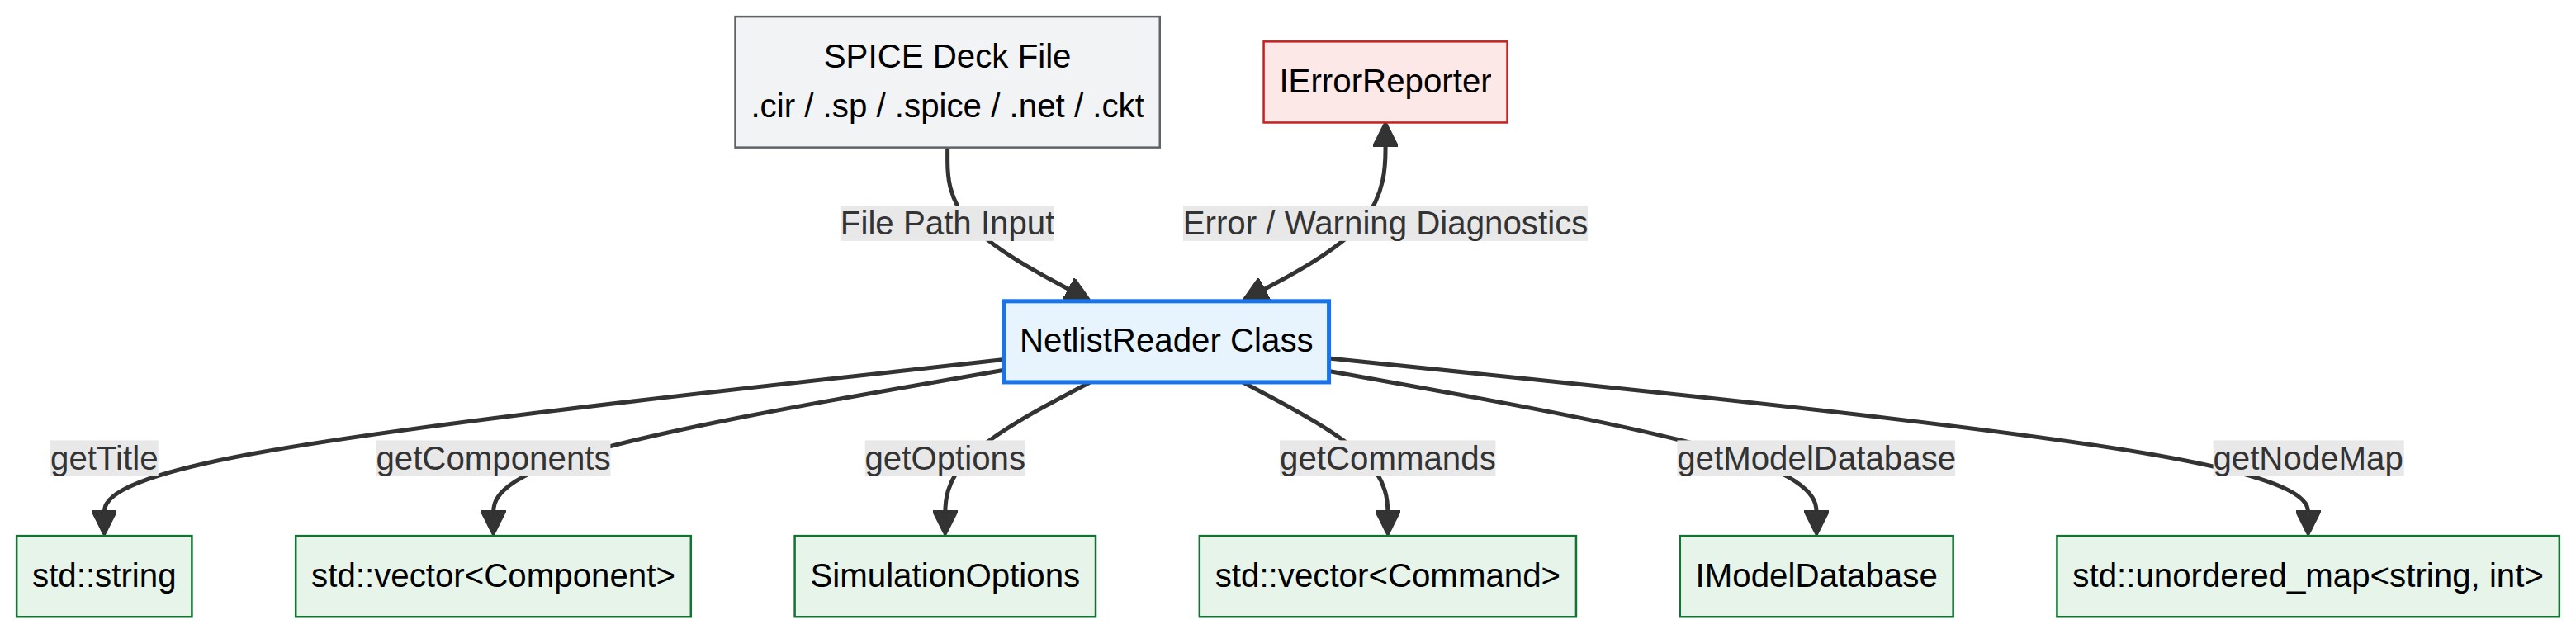
\includegraphics[width=0.85\textwidth]{Figures/Ch4/interface.png}%
}{%
  \framebox[\textwidth][c]{\rule{0pt}{3cm}\textbf{Figure Placeholder: interface.png}}%
}
\caption{System interface block diagram illustrating data interaction between input CAD decks, the NetlistReader facade controller, and downstream solver matrices.}
\label{fig:interface_diagram}
\end{figure}

\subsubsection{Modular Decomposition and Inter-Module Dataflows}

To manage the complexity of lexical analysis, macro expansion, and semantic validation, the internal processing flow is decomposed into specialized, decoupled components. Figure~\ref{fig:detailed_architecture} depicts the detailed architectural layout and inter-module communications within the subsystem. The operational pipeline follows a structured pipe-and-filter pattern:
\begin{enumerate}
    \item \textbf{Stream Validation and Pre-processing}: The flow begins with \texttt{NetlistFileOpener}, which verifies physical file paths and opens the input stream. It streams its output directly to \texttt{NetlistPrepass}, which strips comments, concatenates continuation lines, and extracts the deck title.
    \item \textbf{Lexical Routing}: \texttt{NetlistPrepass} feeds the concatenated lines to \texttt{NetlistLexer}. The lexer tokenizes the statements and distributes them into distinct categorized buckets. These buckets are directly routed to their respective parsers (e.g., \texttt{getParams()} to \texttt{ParamParser}, \texttt{getSubcircuits()} to \texttt{SubcktDefParser}, etc.).
    \item \textbf{Subcircuit Expansion}: \texttt{SubcktInstParser} drives the macro expansion process. It expands subcircuit instances utilizing \texttt{SubcktDefParser} and evaluates parameter overrides using \texttt{ParamParser}. The resulting expanded components, device models, and simulation commands are then output to \texttt{CompParser}, \texttt{ModelParser}, and \texttt{CommandParser}, respectively.
    \item \textbf{Semantic Compilation and Helper Connections}: The remaining sub-parsers compile the routed statements into final simulation entities. \texttt{CompParser} leverages \texttt{NodeManager} to map node names to integer indices, while \texttt{ModelParser} registers device models into \texttt{ModelDatabase}. Crucially, nearly all parsers (\texttt{CompParser}, \texttt{ModelParser}, \texttt{CommandParser}, \texttt{OptionParser}, and \texttt{ParamParser}) rely heavily on \texttt{ValueParser} as a central helper for evaluating mathematical expressions and numeric values.
\end{enumerate}

\begin{figure}[H]
\centering
\IfFileExists{Figures/Ch4/detailed_architecture.png}{%
  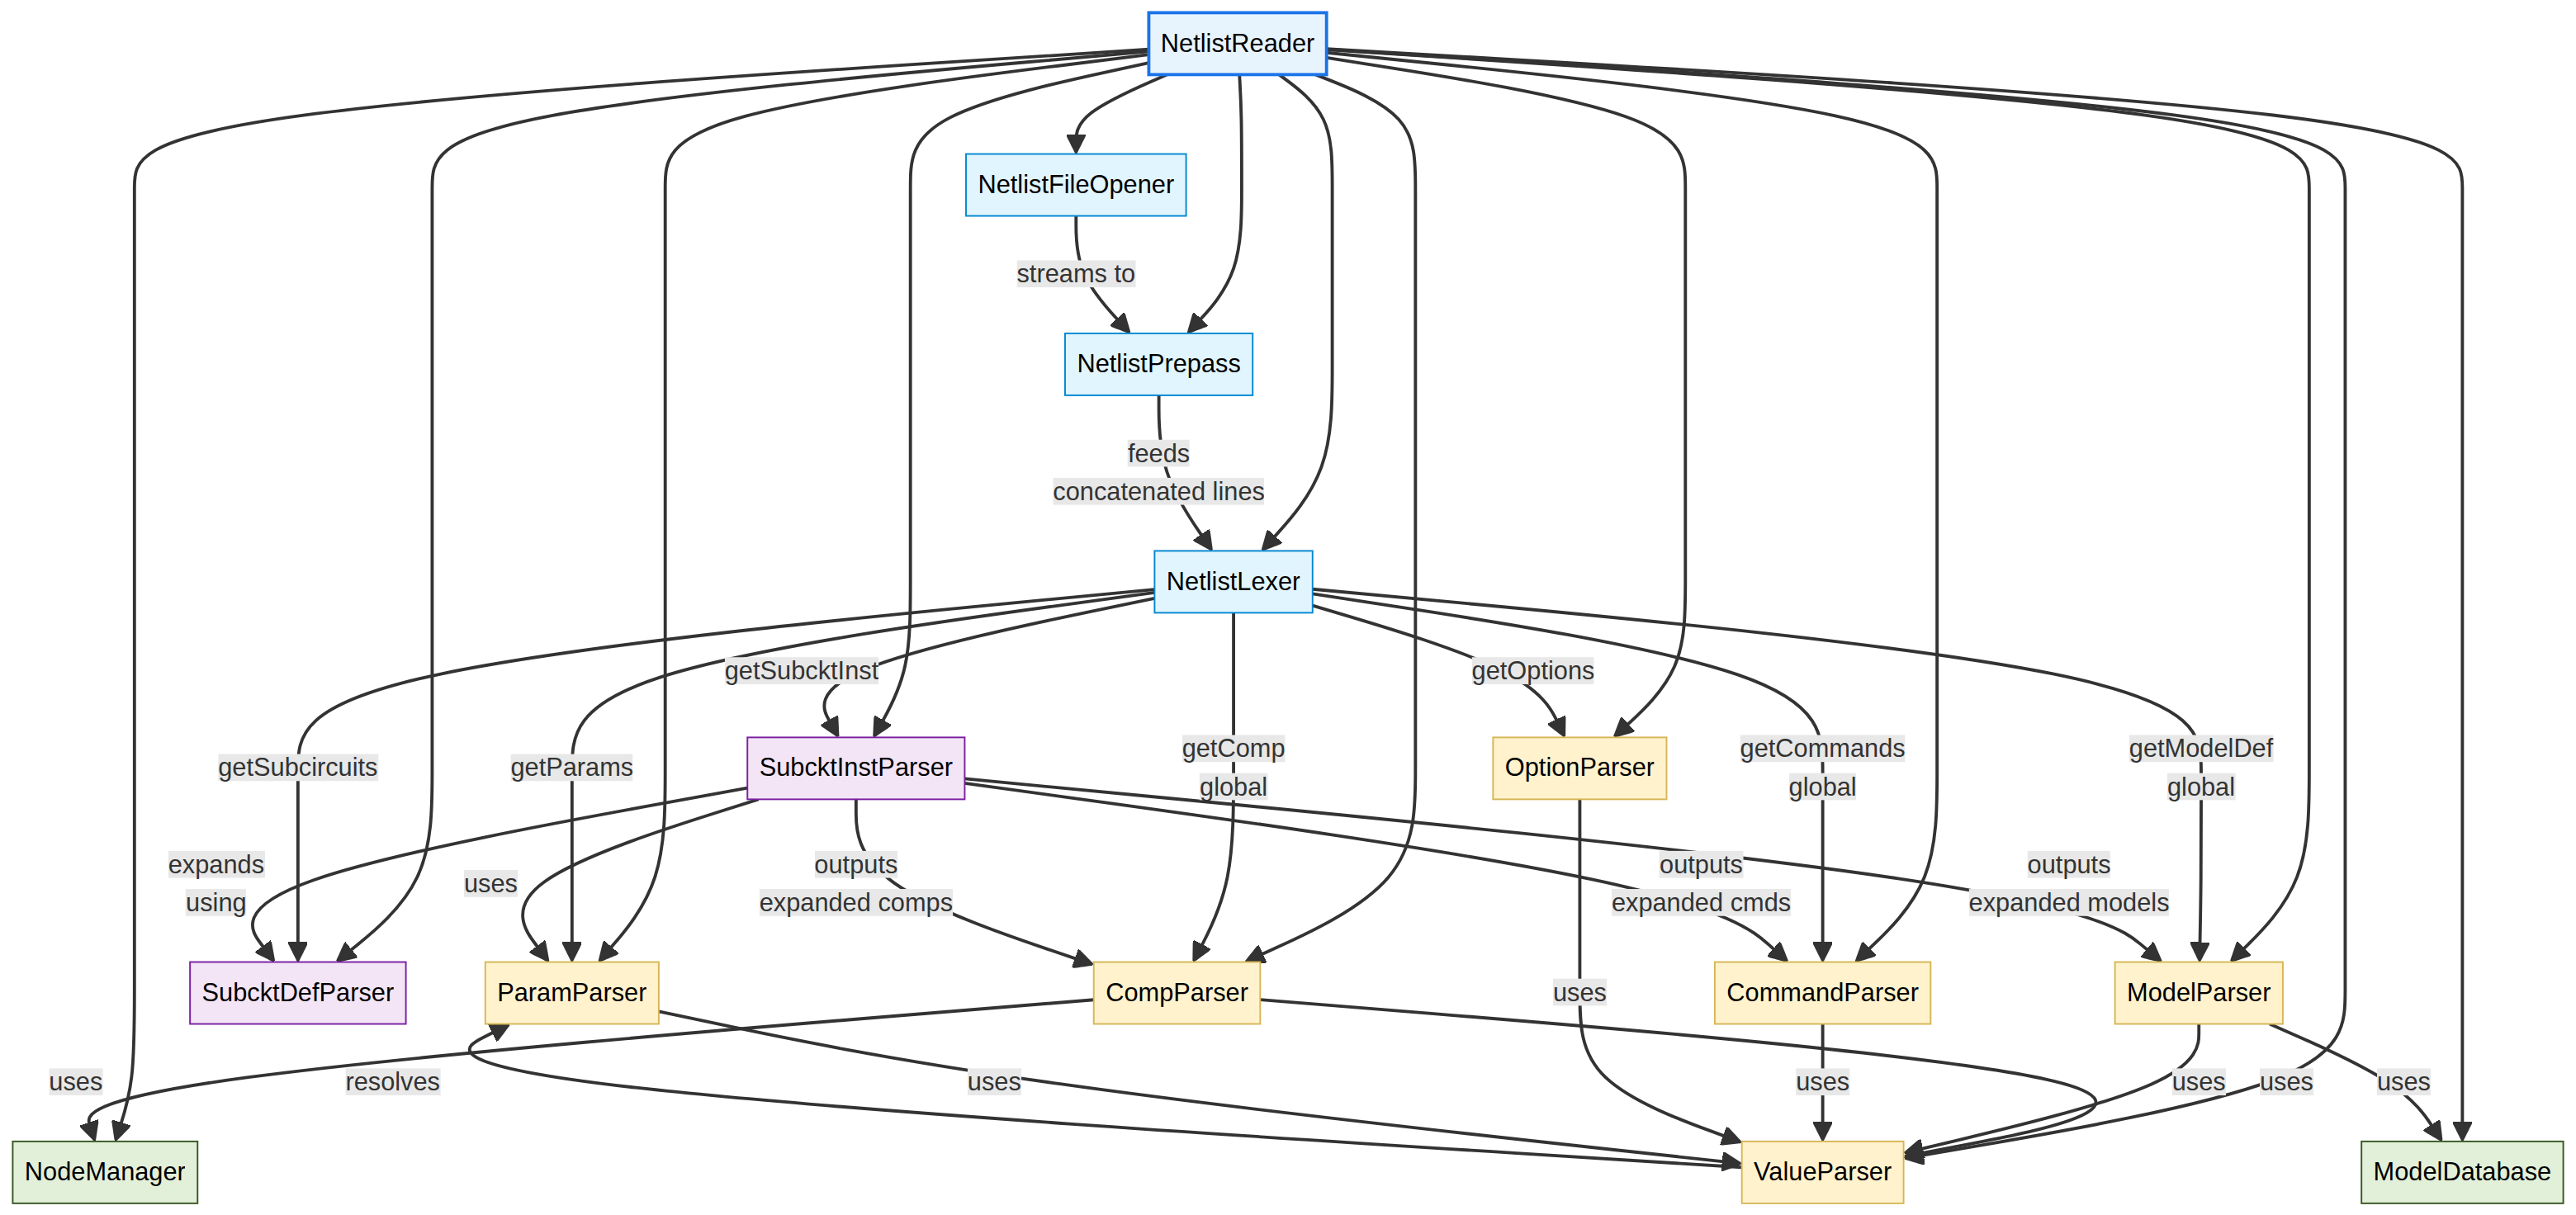
\includegraphics[width=0.9\textwidth]{Figures/Ch4/detailed_architecture.png}%
}{%
  \framebox[\textwidth][c]{\rule{0pt}{3cm}\textbf{Figure Placeholder: detailed_architecture.png}}%
}
\caption{Detailed architectural decomposition illustrating communication and data flow across specialized parsing components.}
\label{fig:detailed_architecture}
\end{figure}

\subsubsection{NetlistReader Execution Flowchart and Processing Control}

The step-by-step operational algorithm and decision logic executed within \texttt{NetlistReader::read()} are detailed in the execution flowchart shown in Figure~\ref{fig:execution_flowchart}. The flowchart traces the exact control logic from initial deck ingestion to final compilation status verification:
\begin{enumerate}
    \item \textbf{State Reset and Isolation}: Execution begins by resetting and clearing all internal components and persistent databases. This enforces strict state isolation between consecutive runs.
    \item \textbf{File Ingestion \& Prepass}: \texttt{NetlistFileOpener} opens a stream for the file path. If the stream cannot be opened, compilation terminates immediately and returns \texttt{false}. Otherwise, \texttt{NetlistPrepass} joins continuation lines and strips comments.
    \item \textbf{Tokenization and Bucket Partitioning}: \texttt{NetlistLexer} tokenizes logical statements and groups them into categorized buckets before routing.
    \item \textbf{Global Parameters and Options Parsing}: Global \texttt{.param} statements are parsed by the \texttt{ParamParser}, followed by the parsing of simulation options via the \texttt{OptionParser}.
    \item \textbf{Macro Expansion and Subcircuit Resolution}: \texttt{SubcktDefParser} parses subcircuit templates, and \texttt{SubcktInstParser} recursively expands and resolves subcircuit calls.
    \item \textbf{Merging and Semantic Compilation}: Global statements and the subcircuit-expanded statements are merged. Following this, device components, device models, and simulation commands are compiled into typed data structures.
    \item \textbf{Diagnostic Status Verification}: Finally, the flow checks if any errors were reported to the \texttt{IErrorReporter}. If errors occurred, it returns \texttt{false}; otherwise, it returns \texttt{true}, signaling successful compilation.
\end{enumerate}

\begin{figure}[htbp]
\centering
\IfFileExists{Figures/Ch4/flowchart.pdf}{%
  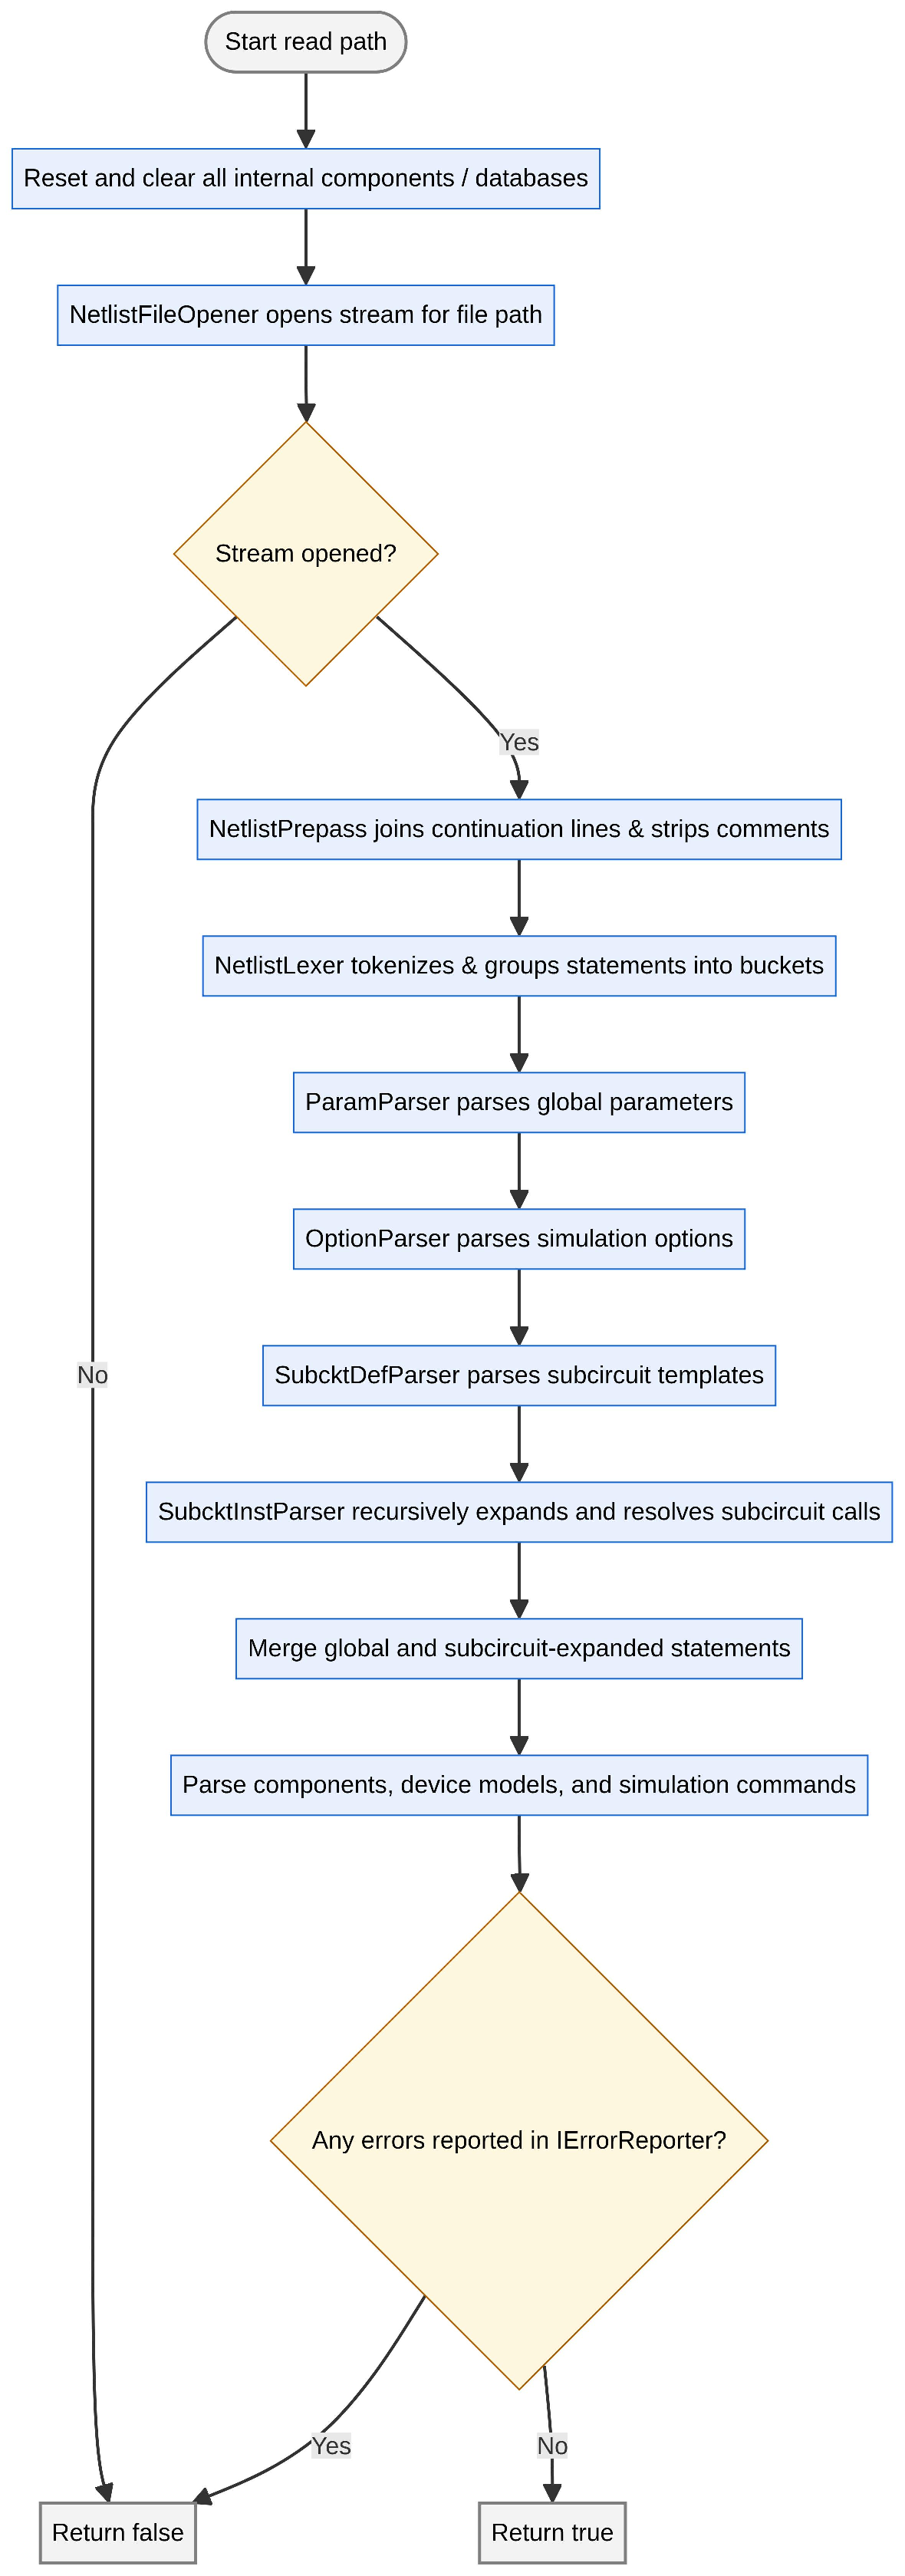
\includegraphics[height=0.8\textheight,keepaspectratio]{Figures/Ch4/flowchart.pdf}%
}{%
  \framebox[\textwidth][c]{\rule{0pt}{3cm}\textbf{Figure Placeholder: flowchart.pdf}}%
}
\caption{Execution flowchart illustrating sequential token routing, macro expansion loops, and semantic validation steps within NetlistReader.}
\label{fig:execution_flowchart}
\end{figure}

\subsubsection{Object-Oriented Architecture and UML Class Relationships}

To provide a comprehensive structural overview of the object-oriented design and interface contracts, Figure~\ref{fig:class_diagram} presents the complete UML class diagram of the subsystem. The diagram highlights core design patterns and software engineering abstractions:
\begin{itemize}
    \item \textbf{Abstract Interface Contracts}: To adhere to the Dependency Inversion Principle (DIP) and Interface Segregation Principle (ISP), high-level parsers interact exclusively through abstract interfaces. Key contracts include \texttt{INetlistReader} (facade interface), \texttt{INodeManager} (node canonicalization), \texttt{IModelDatabase} (model card storage), \texttt{IValueParser} (mathematical formula evaluation), \texttt{ICompParser} (component compilation), \texttt{ICommandParser} (analysis directives), and \texttt{IOptionParser} (simulation controls).
    \item \textbf{Facade and Composition Lifecycles}: \texttt{NetlistReader} acts as the facade controller owning long-lived persistent database managers (\texttt{nodeManager\_}, \texttt{modelDatabase\_}) and core parsers as \texttt{std::unique\_ptr} members to prevent heap reallocation overhead across simulation runs. Transient macro expansion tables (\texttt{SubcktDefParser}, \texttt{SubcktInstParser}) and front-end tools are stack-allocated within \texttt{read()} and automatically reclaimed upon exit.
    \item \textbf{Mutual Dependency Resolution via Two-Phase Binding}: The class diagram illustrates the cyclic dependency between parameter evaluation (\texttt{ParamParser}) and mathematical parsing (\texttt{ValueParser}). This is resolved via deferred two-phase pointer binding: \texttt{ValueParser} receives a raw pointer to \texttt{ParamParser} during construction, followed by explicit back-reference registration via \texttt{setValueParser()}, breaking the initialization cycle cleanly.
\end{itemize}

\begin{sidewaysfigure}
\centering
\IfFileExists{Figures/Ch4/ClassDiagram.pdf}{%
  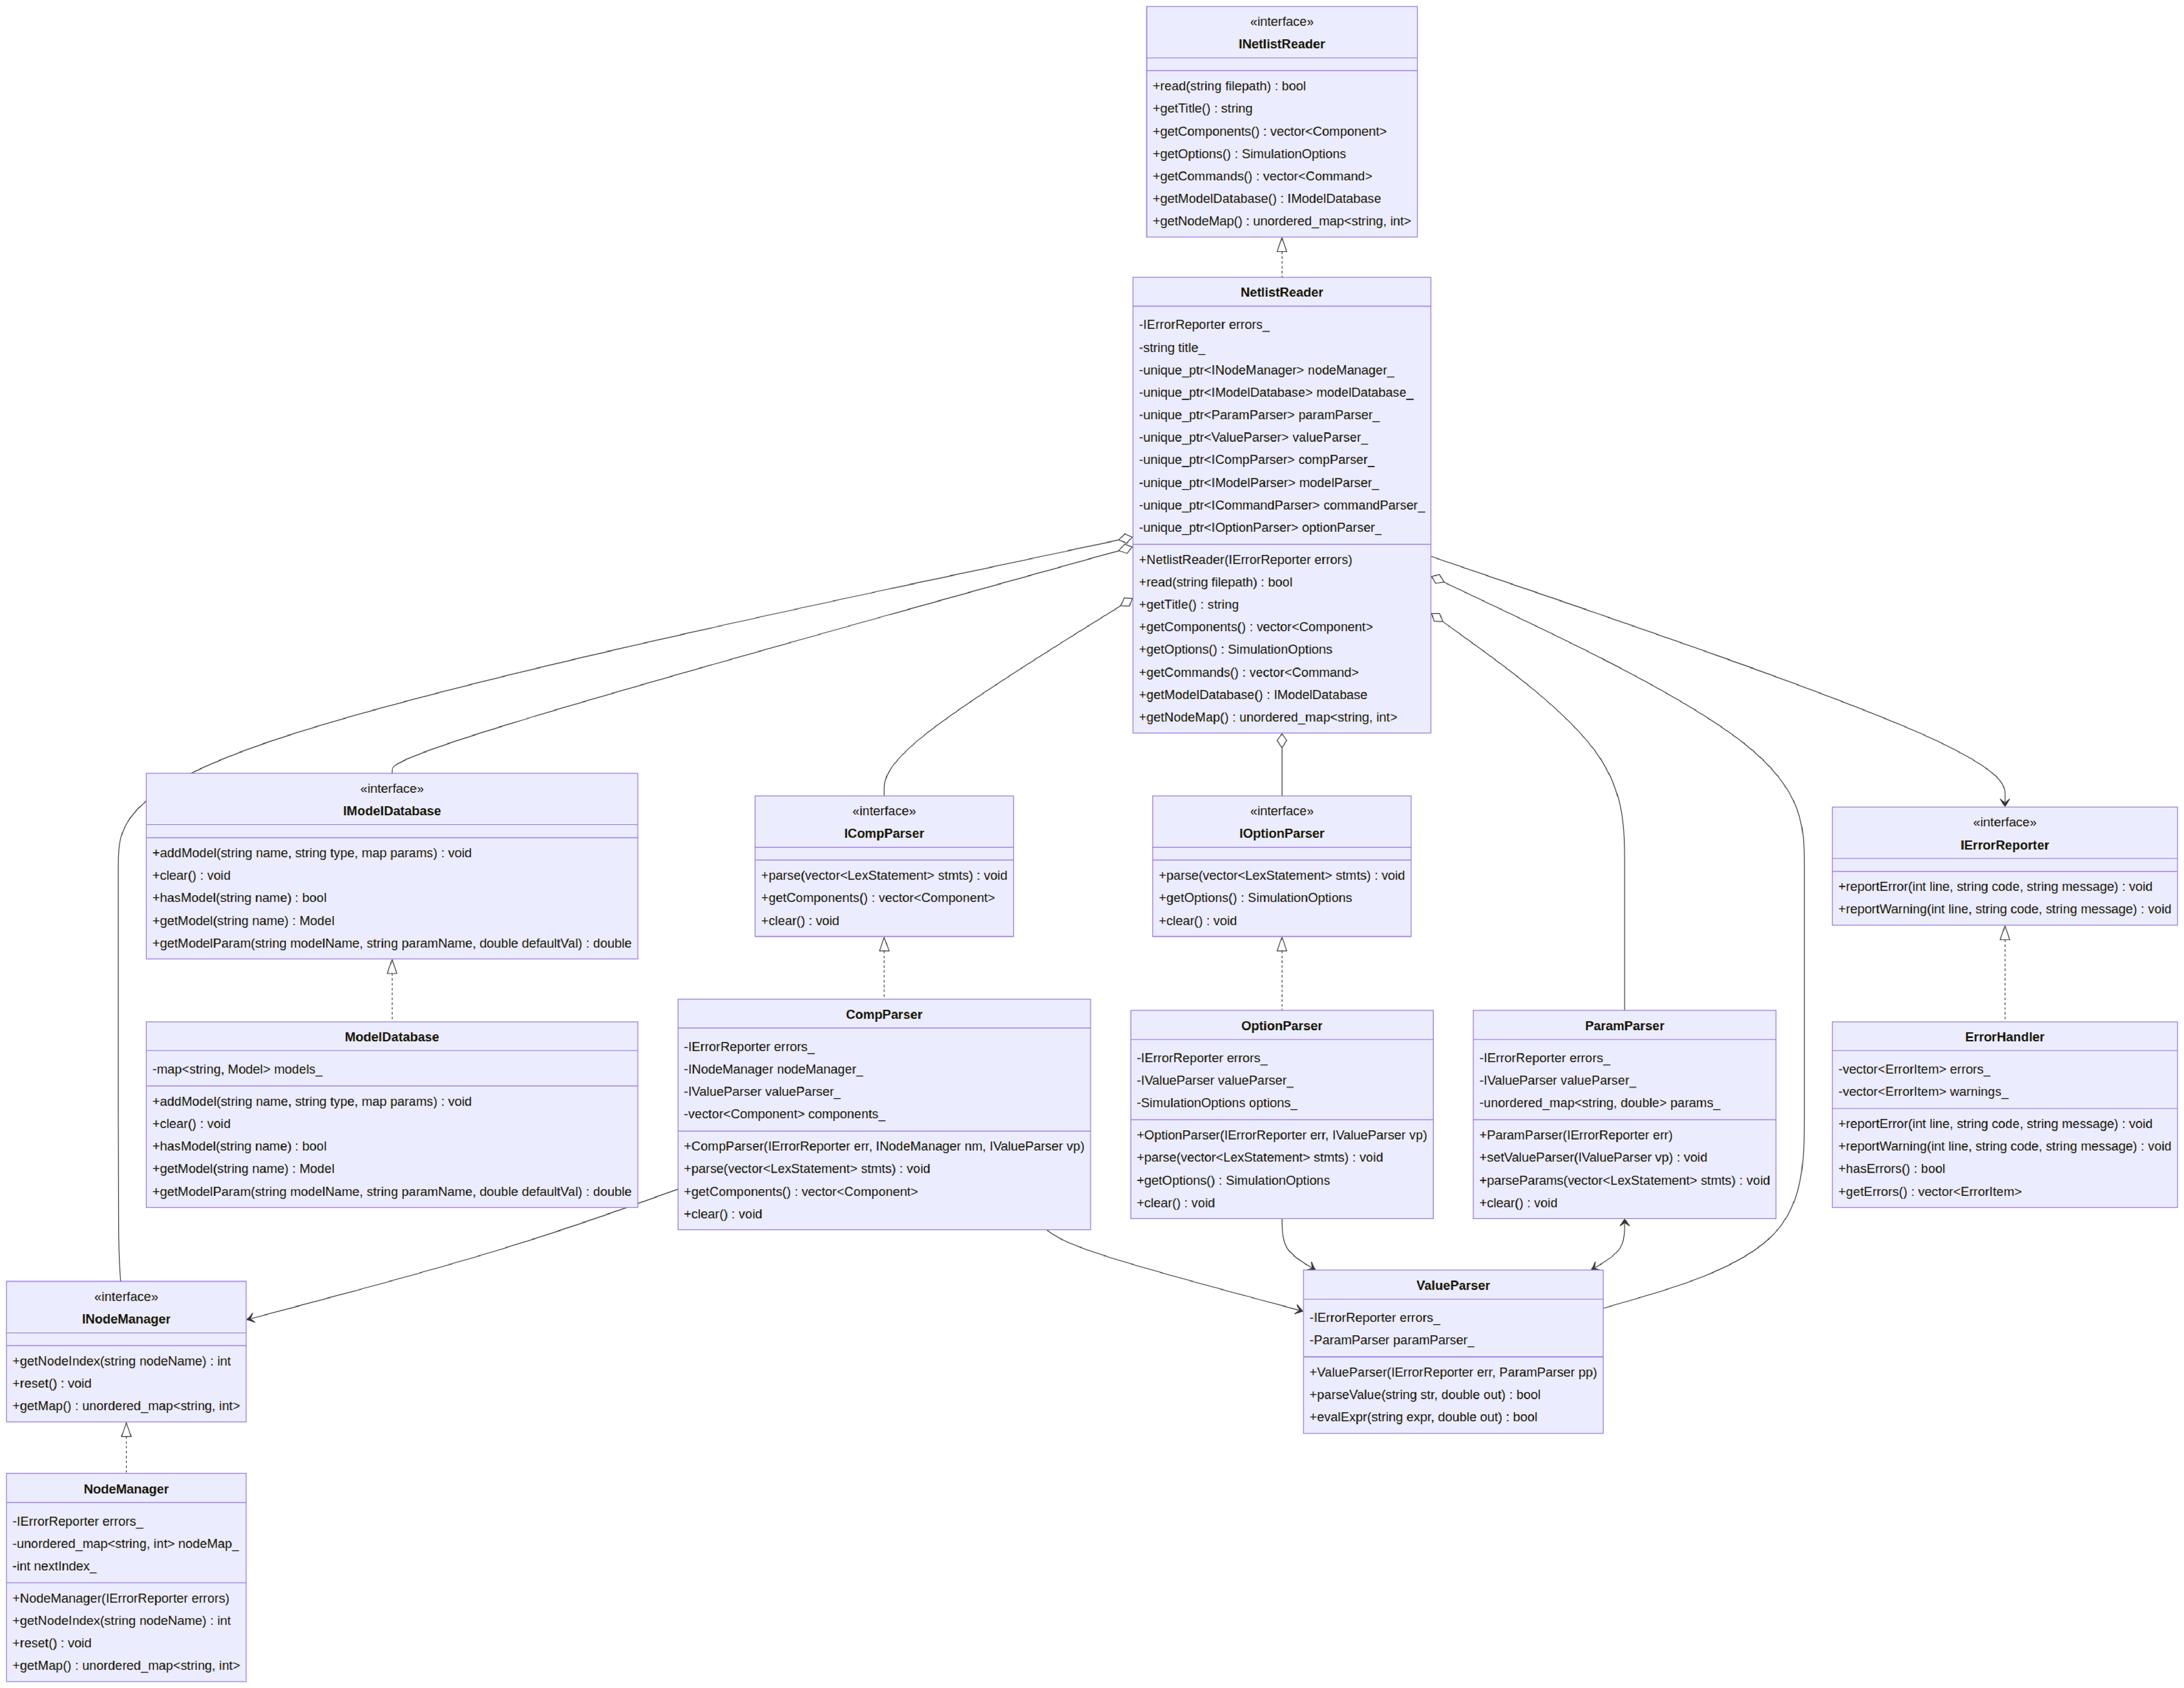
\includegraphics[width=0.95\textheight,height=0.85\textwidth,keepaspectratio]{Figures/Ch4/ClassDiagram.pdf}%
}{%
  \framebox[\textwidth][c]{\rule{0pt}{8cm}\textbf{Figure Placeholder: ClassDiagram.pdf}}%
}
\caption{Complete System UML Class Diagram detailing object-oriented abstractions, inheritance hierarchies, and parser relationships across the subsystem.}
\label{fig:class_diagram}
\end{sidewaysfigure}

The following subsections provide comprehensive documentation for each core class within the subsystem, detailing its primary function, inter-module communications, error models, testing methodology, and test traceability matrices.


\subsection{Module: NetlistReader (Facade Controller)}

\textbf{Function and Purpose:} \texttt{NetlistReader} serves as the top-level controller and facade for the netlist processing pipeline, implementing the \texttt{INetlistReader} interface. It orchestrates multi-stage compilation flow, coordinating file validation, lexical prepass, tokenization, subcircuit flattening, parameter evaluation, and semantic compilation of components, device models, options, and commands.

\textbf{Inter-Module Communication:} Implements \texttt{INetlistReader} and interacts with downstream simulation engines. Internally, it manages the lifecycles of \texttt{NetlistFileOpener}, \texttt{NetlistPrepass}, \texttt{NetlistLexer}, \texttt{ParamParser}, \texttt{OptionParser}, \texttt{SubcktDefParser}, \texttt{SubcktInstParser}, \texttt{CompParser}, \texttt{ModelParser}, and \texttt{CommandParser}.

\textbf{Comprehensive Error Models and Diagnostic Codes:}
\begin{compactitem}
    \item \texttt{FILE\_NOT\_FOUND} / \texttt{FILE\_OPEN\_FAILED}: Raised when the physical path does not exist or stream initialization fails.
    \item \texttt{WRONG\_FILE\_FORMAT} / \texttt{FILE\_INVALID\_EXTENSION}: Raised when deck file extension is not supported.
    \item \texttt{FILE\_EMPTY}: Raised when zero bytes are read from input stream.
    \item \texttt{IErrorReporter} Status Intercept: Queries injected reporter; returns \texttt{false} if any syntactic or semantic errors occurred.
\end{compactitem}

\textbf{Testing Methodology and Complete Traceability Matrix:} Tested using unit tests in \texttt{NetlistReaderTests} and end-to-end integration suites.

\begin{table}[H]
\centering
\small
\begin{tabular}{|l|l|p{4.5cm}|p{4.5cm}|}
\hline
\textbf{Test ID} & \textbf{Test Scenario} & \textbf{Input Setup / Method} & \textbf{Expected Result} \\
\hline
UT-NR-01 & Nonexistent File & \texttt{read("missing.cir")} & Returns \texttt{false}; logs file open error. \\
\hline
UT-NR-02 & Empty File Check & \texttt{read("empty.cir")} & Returns \texttt{false}; logs empty file error. \\
\hline
UT-NR-03 & Extension Check & \texttt{read("deck.txt")} & Returns \texttt{false} (restricts to valid extensions). \\
\hline
UT-NR-04 & State Isolation & Sequential \texttt{read(fileA)} then \texttt{read(fileB)} & Second run contains only \texttt{fileB} components. \\
\hline
UT-NR-05 & Defaults Query & Query \texttt{getParameter} for unpassed option & Returns static registry default value. \\
\hline
UT-NR-06 & Title Capture & Read deck starting with comment title & \texttt{getTitle()} returns trimmed first line string. \\
\hline
UT-NR-07 & Empty Title & Read deck starting with blank line & \texttt{getTitle()} returns empty string. \\
\hline
IT-NR-01 & Semantic Propagation & Subcircuit terminal count mismatch & Returns \texttt{false}; records semantic error. \\
\hline
IT-NR-02 & Empty Subcircuit & Subcircuit containing no devices & Returns \texttt{true}; component DB is empty. \\
\hline
IT-NR-03 & Controls Only & Deck with options and tran analysis only & Returns \texttt{true}; commands and options parsed. \\
\hline
IT-NR-04 & Dependent Sources & Subcircuit CCCS referencing local \texttt{Vmeas} & Controlling source renamed to \texttt{Vmeas:X1}. \\
\hline
IT-NR-05 & Multi Instance & Filter subcircuit instantiated twice & Two independent R-C pairs generated. \\
\hline
IT-NR-06 & Scoping Shadowing & Nested parent/child parameter overrides & Resolves scoped parameters without collision. \\
\hline
IT-NR-07 & Full Deck & Full deck with models, params, commands & Parses deck matching target spec. \\
\hline
\end{tabular}
\caption{Complete Test Traceability Matrix for NetlistReader Controller}
\end{table}


\subsection{Module: NetlistFileOpener (File Access and Validation)}

\textbf{Function and Purpose:} \texttt{NetlistFileOpener} manages stream creation and path validation. It verifies file existence, enforces allowed extension constraints (\texttt{.cir}, \texttt{.sp}, \texttt{.spice}, \texttt{.net}, \texttt{.ckt}), and opens an isolated \texttt{std::ifstream} handle for pre-processing.

\textbf{Inter-Module Communication:} Invoked by \texttt{NetlistReader} during initialization, reporting diagnostic events directly to \texttt{IErrorReporter}.

\textbf{Comprehensive Error Models and Diagnostic Codes:}
\begin{compactitem}
    \item \texttt{WRONG\_FILE\_FORMAT}: Extension is not in the supported set (case-insensitive check).
    \item \texttt{FILE\_OPEN\_FAILED}: Stream could not be opened due to missing path or access restriction.
    \item \texttt{EMPTY\_FILE}: Zero bytes read from stream handle.
\end{compactitem}

\textbf{Testing Methodology and Complete Traceability Matrix:} Tested using temporary real files in system temp directory via \texttt{NetlistFileOpenerTests}.

\begin{table}[H]
\centering
\small
\begin{tabular}{|l|l|p{4.5cm}|p{4.5cm}|}
\hline
\textbf{Test ID} & \textbf{Test Scenario} & \textbf{Input Setup / Method} & \textbf{Expected Result} \\
\hline
TC-FO-01 & Wrong Extension & Path ending in \texttt{.txt} & \texttt{open} returns \texttt{nullptr}; code \texttt{WRONG\_FILE\_FORMAT}. \\
\hline
TC-FO-02 & Open Failure & Nonexistent \texttt{.cir} path & \texttt{open} returns \texttt{nullptr}; code \texttt{FILE\_OPEN\_FAILED}. \\
\hline
TC-FO-03 & Empty File & Existing zero-byte \texttt{.cir} file & \texttt{open} returns \texttt{nullptr}; code \texttt{EMPTY\_FILE}. \\
\hline
TC-FO-04 & Valid Netlist & Non-empty \texttt{.cir} file & Returns valid stream; line 1 readable; no errors. \\
\hline
TC-FO-05 & Case Insensitive & Non-empty \texttt{.CIR} file & Returns valid stream; no errors. \\
\hline
\end{tabular}
\caption{Complete Test Traceability Matrix for NetlistFileOpener}
\end{table}


\subsection{Module: NetlistPrepass (Logical Normalization)}

\textbf{Functionality and Purpose:} \texttt{NetlistPrepass} normalizes raw line streams into logical statements. It extracts the deck title from line 1, strips full-line (\texttt{*}) and inline (\texttt{;}, \texttt{//}) comments, and joins line continuation sequences (\texttt{+}) while preserving line mappings.

\textbf{Inter-Module Communication:} Consumes input stream from \texttt{NetlistFileOpener} and passes clean logical lines to \texttt{NetlistLexer}.

\textbf{Comprehensive Error Models and Diagnostic Codes:}
\begin{compactitem}
    \item \texttt{CONTINUATION\_ERROR}: Raised when a continuation character (\texttt{+}) appears on the very first physical line or before any logical statement has been established.
\end{compactitem}

\textbf{Testing Methodology and Complete Traceability Matrix:} Tested using in-memory streams and fake error reporters in \texttt{NetlistPrepassTests}.

\begin{table}[H]
\centering
\small
\begin{tabular}{|l|l|p{4.5cm}|p{4.5cm}|}
\hline
\textbf{Test ID} & \textbf{Test Scenario} & \textbf{Input Setup / Method} & \textbf{Expected Result} \\
\hline
TC-PP-01 & Title Capture & Line 1 contains text & \texttt{title} equals line 1 text; excluded from lines list. \\
\hline
TC-PP-02 & Blank Title & Line 1 is blank & \texttt{title} is empty string; later text parsed into lines. \\
\hline
TC-PP-03 & Inline Comments & Statements with \texttt{\#}, \texttt{;}, \texttt{//} & Comment suffix removed from logical statement text. \\
\hline
TC-PP-04 & Continuation Join & Statement followed by \texttt{+} line & Continuation appended to prior logical statement. \\
\hline
TC-PP-05 & Orphan Continuation & \texttt{+} line before any statement & Emits \texttt{CONTINUATION\_ERROR} at source line. \\
\hline
\end{tabular}
\caption{Complete Test Traceability Matrix for NetlistPrepass}
\end{table}


\subsection{Module: NetlistLexer (Lexical Analysis \& Statement Routing)}

\textbf{Functionality and Purpose:} \texttt{NetlistLexer} performs lexical categorization, partitioning logical lines into discrete tokens (\texttt{LexToken}) and categorizing statements into functional buckets (\texttt{LexStatement} and \texttt{LexSubcircuit}).

\textbf{Inter-Module Communication:} Populates statement vectors consumed by \texttt{ParamParser}, \texttt{OptionParser}, \texttt{SubcktDefParser}, \texttt{CompParser}, \texttt{ModelParser}, and \texttt{CommandParser}.

\textbf{Comprehensive Error Models and Diagnostic Codes:}
\begin{compactitem}
    \item \texttt{UNTERMINATED\_QUOTE}: Missing closing quote for string token.
    \item \texttt{UNTERMINATED\_BRACE\_EXPR}: Missing closing brace for mathematical expression.
    \item \texttt{CONTROL\_BLOCK\_ERROR}: Nested \texttt{.control} blocks or orphan \texttt{.endc}.
    \item \texttt{SYNTAX\_ERROR}: \texttt{.control} or \texttt{.endc} directive provided with extra arguments.
    \item \texttt{CTRL\_DOT\_SYNTAX}: Statement inside \texttt{.control} block starts with a leading dot.
    \item \texttt{CTRL\_DISALLOWED\_SUBCKT}: Subcircuit directive inside \texttt{.control} block.
    \item \texttt{CTRL\_DISALLOWED\_COMPONENT\_DEF}: Component definition inside \texttt{.control} block.
    \item \texttt{CTRL\_DISALLOWED\_DECK\_DIRECTIVE}: Deck directive (\texttt{model}, \texttt{param}, \texttt{options}) inside \texttt{.control}.
    \item \texttt{CONTROL\_INSIDE\_SUBCKT}: \texttt{.control} block declared inside a subcircuit definition.
    \item \texttt{NESTED\_SUBCKT}: Subcircuit definition nested inside another subcircuit.
    \item \texttt{ENDS\_WITHOUT\_SUBCKT}: \texttt{.ends} directive encountered without preceding \texttt{.subckt}.
    \item \texttt{UNKNOWN\_STATEMENT}: Unrecognized statement head outside control blocks or inside subcircuits.
    \item \texttt{UNCLOSED\_CONTROL} / \texttt{UNCLOSED\_SUBCKT}: Block unclosed at end of input deck.
    \item \texttt{SUBCKT\_DISALLOWED\_OPTIONS}: Options statement placed inside a subcircuit block.
    \item \texttt{AFTER\_END\_IGNORED} (Warning): Statements present after \texttt{.end} are ignored.
\end{compactitem}

\textbf{Testing Methodology and Complete Traceability Matrix:} Tested via token classification and statement routing validation in \texttt{NetlistLexerTests}.

\begin{table}[H]
\centering
\small
\begin{tabular}{|l|l|p{4.5cm}|p{4.5cm}|}
\hline
\textbf{Test ID} & \textbf{Test Scenario} & \textbf{Input Setup / Method} & \textbf{Expected Result} \\
\hline
TC-LX-01 & Param Routing & \texttt{.param res=1k} & Routed to params bucket; dot stripped. \\
\hline
TC-LX-02 & Comp Routing & \texttt{R1 1 0 1k} & Routed to comp bucket. \\
\hline
TC-LX-03 & Brace Token & \texttt{C1 1 0 \{2u*gain\}} & Kept as single expression token. \\
\hline
TC-LX-04 & Nested Brace & \texttt{R1 1 0 \{a+\{b*c\}\}} & Tokenized as single expression token. \\
\hline
TC-LX-05 & Unterminated Brace & \texttt{R1 1 0 \{a+b} & Emits \texttt{UNTERMINATED\_BRACE\_EXPR}. \\
\hline
TC-LX-06 & Quoted Token & \texttt{R1 1 0 "str"} & Tokenized with \texttt{quoted=true}. \\
\hline
TC-LX-07 & Unterminated Quote & \texttt{R1 1 0 "str} & Emits \texttt{UNTERMINATED\_QUOTE}. \\
\hline
TC-LX-08 & Control Dot Syntax & \texttt{.control} then \texttt{.op} & Emits \texttt{CTRL\_DOT\_SYNTAX}. \\
\hline
TC-LX-09 & Control Comp Def & \texttt{.control} then \texttt{R1 1 0 1k} & Emits \texttt{CTRL\_DISALLOWED\_COMPONENT\_DEF}. \\
\hline
TC-LX-10 & Control Directive & \texttt{.control} then \texttt{param x=1} & Emits \texttt{CTRL\_DISALLOWED\_DECK\_DIRECTIVE}. \\
\hline
TC-LX-11 & Unclosed Control & \texttt{.control} without \texttt{.endc} & Emits \texttt{UNCLOSED\_CONTROL}. \\
\hline
TC-LX-12 & After End Ignored & Statements after \texttt{.end} & Ignored; emits \texttt{AFTER\_END\_IGNORED} warning. \\
\hline
TC-LX-13 & Valid Subcircuit & \texttt{.subckt sub 1 2} ... \texttt{.ends} & Subcircuit block collected cleanly into subcircuits vector. \\
\hline
TC-LX-14 & Nested Subcircuit & \texttt{.subckt s1} then \texttt{.subckt s2} & Emits \texttt{NESTED\_SUBCKT}. \\
\hline
TC-LX-15 & Subckt in Control & \texttt{.control} then \texttt{subckt s1} & Emits \texttt{CTRL\_DISALLOWED\_SUBCKT}. \\
\hline
TC-LX-16 & Control in Subckt & \texttt{.subckt s1} then \texttt{.control} & Emits \texttt{CONTROL\_INSIDE\_SUBCKT}. \\
\hline
TC-LX-17 & Unclosed Subckt EOF & \texttt{.subckt s1} without \texttt{.ends} & Emits \texttt{UNCLOSED\_SUBCKT}. \\
\hline
TC-LX-18 & Unclosed Subckt END & \texttt{.subckt s1} then \texttt{.end} & Emits \texttt{UNCLOSED\_SUBCKT}. \\
\hline
TC-LX-19 & Ends without Subckt & \texttt{.ends} without opening & Emits \texttt{ENDS\_WITHOUT\_SUBCKT}. \\
\hline
TC-LX-20 & Equals Space Norm & \texttt{M1 1 2 3 4 model w = 10u} & Merges into single token \texttt{"w=10u"}. \\
\hline
TC-LX-21 & Unknown Subckt Stmt & \texttt{.subckt s1} then \texttt{Y1 1 2} & Emits \texttt{UNKNOWN\_STATEMENT}. \\
\hline
TC-LX-22 & Instance Routing & \texttt{X1 1 2 sub1} & Routed to \texttt{subcktInst} bucket. \\
\hline
TC-LX-23 & Options Routing & \texttt{.options temp=25} & Routed to options bucket; dot stripped. \\
\hline
TC-LX-24 & Options in Subckt & \texttt{.subckt s1} then \texttt{.options} & Emits \texttt{SUBCKT\_DISALLOWED\_OPTIONS}. \\
\hline
TC-LX-25 & Commands Order & Multiple commands in deck & Commands stored in sequential order. \\
\hline
TC-LX-26 & Subckt Commands & Commands inside subcircuit & Subcircuit commands collected in order. \\
\hline
TC-LX-27 & Generalized Cmds & Dotted outside / dotless inside & Routed to commands bucket without error. \\
\hline
\end{tabular}
\caption{Complete Test Traceability Matrix for NetlistLexer}
\end{table}


\subsection{Module: ParamParser (Parameter Expression Resolution)}

\textbf{Functionality and Purpose:} \texttt{ParamParser} parses global and local \texttt{.param} assignments, managing symbolic parameter evaluation and cross-parameter reference inheritance across hierarchical scopes.

\textbf{Inter-Module Communication:} Interacts with \texttt{ValueParser} for expression evaluation and provides resolved parameter lookup tables to \texttt{SubcktInstParser}.

\textbf{Comprehensive Error Models and Diagnostic Codes:}
\begin{compactitem}
    \item \texttt{PARAM\_SYNTAX\_ERROR}: Syntax errors in parameter lines (missing \texttt{=}, too few tokens, or missing assignment expression).
    \item \texttt{PARAM\_UNDEFINED}: Attempting to retrieve a value for an undefined parameter identifier.
    \item \texttt{VALUE\_ERROR}: Circular dependency detected during evaluation (e.g., \texttt{a=\{b\}}, \texttt{b=\{a\}}).
    \item \texttt{PARAM\_ERROR}: Attempting to evaluate parameter values when \texttt{IValueParser} back-reference has not been bound.
\end{compactitem}

\textbf{Testing Methodology and Complete Traceability Matrix:} Tested using mock value parsers in \texttt{ParamParserTests}.

\begin{table}[H]
\centering
\small
\begin{tabular}{|l|l|p{4.5cm}|p{4.5cm}|}
\hline
\textbf{Test ID} & \textbf{Test Scenario} & \textbf{Input Setup / Method} & \textbf{Expected Result} \\
\hline
TC-PR-01 & Simple Parameter & \texttt{param r\_val = 1k} & \texttt{hasParameter} is true; returns \texttt{1000.0}. \\
\hline
TC-PR-02 & Case Insensitivity & \texttt{param My\_Val = 42} & Case-insensitive lookup (both \texttt{my\_val} and \texttt{MY\_VAL} match). \\
\hline
TC-PR-03 & Param Dependency & \texttt{param base=100} then \texttt{param der=\{base*2\}} & Resolves \texttt{der} to \texttt{200.0}. \\
\hline
TC-PR-04 & Circular Dependency & \texttt{param a=\{b\}}, \texttt{param b=\{a\}} & Reports \texttt{VALUE\_ERROR} during evaluation. \\
\hline
TC-PR-05 & Undefined Param & Accessing \texttt{nonexistent} & Reports \texttt{PARAM\_UNDEFINED}; returns \texttt{0.0}. \\
\hline
TC-PR-06 & Missing Equals & \texttt{param x 5} & Reports \texttt{PARAM\_SYNTAX\_ERROR}. \\
\hline
TC-PR-07 & Too Few Tokens & \texttt{param x} & Reports \texttt{PARAM\_SYNTAX\_ERROR}. \\
\hline
TC-PR-08 & No Value Parser & Evaluating without setting ValueParser & Reports \texttt{PARAM\_ERROR}; returns \texttt{0.0}. \\
\hline
TC-PR-09 & Clear Parameters & Calling \texttt{clear()} protocol & All defined parameters are cleared. \\
\hline
TC-PR-10 & Overwrite Definition & Defining same parameter twice & Latest expression stored; cached value invalidated. \\
\hline
\end{tabular}
\caption{Complete Test Traceability Matrix for ParamParser}
\end{table}


\subsection{Module: ValueParser (Formula Evaluation \& Engineering Units)}

\textbf{Functionality and Purpose:} \texttt{ValueParser} implements mathematical string parsing, converting engineering scale suffixes (\texttt{k}, \texttt{u}, \texttt{m}, \texttt{meg}, \texttt{p}, \texttt{f}) and curly-brace expressions into double-precision numeric values.

\textbf{Inter-Module Communication:} Implements \texttt{IValueParser}. Injected into semantic parsers and maintains a two-phase pointer binding with \texttt{ParamParser}.

\textbf{Comprehensive Error Models and Diagnostic Codes:}
\begin{compactitem}
    \item \texttt{VALUE\_ERROR}: Empty or whitespace value string; missing numeric prefix in plain literal; division by zero; empty brace expression; unexpected token at end of expression; unterminated parenthesis; nested curly braces; undefined parameter during evaluation.
    \item \texttt{VALUE\_WARN}: Trailing suffix starts with unrecognized multiplier prefix (defaults to scale factor \texttt{1.0}).
\end{compactitem}

\textbf{Testing Methodology and Complete Traceability Matrix:} Tested via unit test suite \texttt{ValueParserTests} and integration suite \texttt{ValueParserIntegrationTests}.
\newpage
\begin{table}[H]
\centering
\small
\begin{tabular}{|l|l|p{4.5cm}|p{4.5cm}|}
\hline
\textbf{Test ID} & \textbf{Test Scenario} & \textbf{Input Setup / Method} & \textbf{Expected Result} \\
\hline
TC-VP-01 & Plain Numerics & \texttt{"10"}, \texttt{"3.5"}, \texttt{"1e-3"} & Parsed correctly; no warnings/errors. \\
\hline
TC-VP-02 & Optional Sign & \texttt{"+10"}, \texttt{"-10"}, \texttt{"-1e3"} & Parsed correctly; no warnings/errors. \\
\hline
TC-VP-03 & Whitespace & \texttt{"   10   "}, \texttt{"\textbackslash t-3.5k  "} & Parsed correctly; whitespace ignored. \\
\hline
TC-VP-04 & Single Suffixes & \texttt{"1t"}, \texttt{"1k"}, \texttt{"1u"}, \texttt{"1f"} & Scaled by correct engineering multiplier. \\
\hline
TC-VP-05 & Meg Suffix & \texttt{"2meg"}, \texttt{"2MEG"}, \texttt{"2Meg"} & Scaled to \texttt{2e6}. \\
\hline
TC-VP-06 & Trailing Units & \texttt{"10uF"}, \texttt{"1kHz"}, \texttt{"-3mA"} & Units stripped; correctly scaled values. \\
\hline
TC-VP-07 & Unknown Suffix & \texttt{"10X"} & Emits \texttt{VALUE\_WARN}; value unscaled. \\
\hline
TC-VP-08 & Empty Input & \texttt{""}, \texttt{"   "} & Emits \texttt{VALUE\_ERROR}; returns \texttt{0.0}. \\
\hline
TC-VP-09 & Invalid Prefix & \texttt{"abc"}, \texttt{"k10"} & Emits \texttt{VALUE\_ERROR}; returns \texttt{0.0}. \\
\hline
TC-VP-10 & Exponent Digits & \texttt{"1e"} & Emits \texttt{VALUE\_WARN}; returns \texttt{1.0}. \\
\hline
TC-VP-11 & UTF-8 Micro & \texttt{"4.7u"} / UTF-8 micro & Scaled to \texttt{4.7e-6}. \\
\hline
TC-VP-12 & Double Decimals & \texttt{"5.4.3"} & Emits \texttt{VALUE\_WARN}; parses \texttt{5.4}. \\
\hline
TC-VP-13 & Double Minus & \texttt{"--4"} & Emits \texttt{VALUE\_ERROR}; returns \texttt{0.0}. \\
\hline
TC-VP-14 & Plus-Minus & \texttt{"+-4"} & Emits \texttt{VALUE\_ERROR}; returns \texttt{0.0}. \\
\hline
TC-VP-15 & Leading Equals & \texttt{"=5"} & Emits \texttt{VALUE\_ERROR}; returns \texttt{0.0}. \\
\hline
TC-VP-16 & Compound Unit & \texttt{"-1.4e7 MegkA"} & Scaled to \texttt{-1.4e13}; no errors. \\
\hline
TC-VP-17 & Brace Expression & \texttt{"\{1.5k + 200\}"} & Evaluates expression to \texttt{1700.0}. \\
\hline
TC-VP-18 & Complex Brace & \texttt{"\{ (2u * 10) + 1.5m \}"} & Evaluates expression to \texttt{0.00152}. \\
\hline
TC-VP-19 & Suffix Outside & \texttt{"\{5 * 5\}meg"} & Evaluates expression and applies \texttt{1e6} multiplier. \\
\hline
TC-VP-20 & Unknown Post-Brace & \texttt{"\{5 * 5\}X"} & Emits \texttt{VALUE\_WARN}; returns \texttt{25.0}. \\
\hline
TC-VP-21 & Math Division & \texttt{"\{ -10k / 2 \}"} & Evaluates expression to \texttt{-5000.0}. \\
\hline
TC-VP-22 & Param Resolve & \texttt{"\{x + y\}"} with \texttt{x=10, y=20} & Resolves parameters to \texttt{30.0}. \\
\hline
TC-VP-23 & Undefined Param & \texttt{"\{unknown + 5\}"} & Emits \texttt{VALUE\_ERROR}. \\
\hline
TC-VP-24 & Missing Provider & \texttt{"\{x + 5\}"} with null provider & Emits \texttt{VALUE\_ERROR}. \\
\hline
TC-VP-25 & Literal Div Zero & \texttt{"\{ 1 / 0 \}"} & Emits \texttt{VALUE\_ERROR}. \\
\hline
TC-VP-26 & Param Div Zero & \texttt{"\{ 1 / freq \}"} with \texttt{freq=0.0} & Emits \texttt{VALUE\_ERROR}. \\
\hline
TC-VP-27 & Nested Braces & \texttt{"\{1 + \{2\}\}"} & Emits \texttt{VALUE\_ERROR}. \\
\hline
TC-VP-28 & Empty Braces & \texttt{"\{\}"} & Emits \texttt{VALUE\_ERROR}. \\
\hline
TC-VP-29 & Unclosed Paren & \texttt{"\{(1+2\}"} & Emits \texttt{VALUE\_ERROR}. \\
\hline
TC-VP-30 & Missing Operand & \texttt{"\{*\}"} & Emits \texttt{VALUE\_ERROR}. \\
\hline
IT-VP-01 & Param Integration & \texttt{.param freq=1meg} evaluated in \texttt{\{freq/2\}} & Resolves to \texttt{500000.0} via \texttt{ParamParser}. \\
\hline
\end{tabular}
\caption{Complete Test Traceability Matrix for ValueParser}
\end{table}


\subsection{Module: OptionParser (Simulation Controls \& Solver Options)}

\textbf{Functionality and Purpose:} \texttt{OptionParser} compiles global \texttt{.options} cards, extracting numerical tolerances (\texttt{RELTOL}, \texttt{ABSTOL}, \texttt{VNTOL}), iteration limits (\texttt{ITL1}--\texttt{4}), integration methods (\texttt{TRAP}, \texttt{BE}, \texttt{GEAR}), and sparse matrix solver selections.

\textbf{Inter-Module Communication:} Implements \texttt{IOptionParser}. Populates \texttt{SimulationOptions} returned by \texttt{NetlistReader::getOptions()}.

\textbf{Comprehensive Error Models and Diagnostic Codes:}
\begin{compactitem}
    \item \texttt{OPTION\_UNKNOWN}: Unrecognized option name specified on card.
    \item \texttt{OPTION\_MISSING\_VALUE}: Option requiring value specified without one.
    \item \texttt{OPTION\_INVALID\_VALUE}: Value cannot be parsed or does not match valid enum/boolean synonyms.
    \item \texttt{OPTION\_INVALID\_SYNTAX}: Empty option key specified on card.
\end{compactitem}

\textbf{Testing Methodology and Complete Traceability Matrix:} Tested using \texttt{OptionParserTests} unit test suite.
\newpage
\begin{table}[H]
\centering
\small
\begin{tabular}{|l|l|p{4.5cm}|p{4.5cm}|}
\hline
\textbf{Test ID} & \textbf{Test Scenario} & \textbf{Input Setup / Method} & \textbf{Expected Result} \\
\hline
TC-OP-01 & Double Tolerances & \texttt{.options reltol=1e-4 abstol=1e-11} & Sets corresponding double tolerances. \\
\hline
TC-OP-02 & Iteration Limits & \texttt{.options itl1=120 itl2=60 itl4=15} & Sets corresponding integer limits. \\
\hline
TC-OP-03 & Integration Method & \texttt{.options method=trap} / \texttt{method=gear} & Sets transient integration enum in options. \\
\hline
TC-OP-04 & Solver Selection & \texttt{.options solver=klu} / \texttt{solver=nicslu} & Sets linear solver enum in options. \\
\hline
TC-OP-05 & Boolean Flags & \texttt{.options verbose} / \texttt{usegminstepping=false} & Resolves boolean flags correctly. \\
\hline
TC-OP-06 & Spacing Separators & \texttt{.options reltol = 1e-4 (abstol=1e-11)} & Cleans visual delimiters and parses options. \\
\hline
TC-OP-07 & Unknown Option & \texttt{.options invalid\_key=5} & Emits \texttt{OPTION\_UNKNOWN} error. \\
\hline
TC-OP-08 & Missing Value & \texttt{.options reltol =} & Emits \texttt{OPTION\_MISSING\_VALUE} error. \\
\hline
TC-OP-09 & Invalid Boolean & \texttt{.options verbose=maybe} & Emits \texttt{OPTION\_INVALID\_VALUE} error. \\
\hline
TC-OP-10 & Invalid Method & \texttt{.options method=rungekutta} & Emits \texttt{OPTION\_INVALID\_VALUE} error. \\
\hline
TC-OP-11 & Invalid Solver & \texttt{.options solver=superlu} & Emits \texttt{OPTION\_INVALID\_VALUE} error. \\
\hline
TC-OP-12 & Empty Key Syntax & \texttt{.options =1e-4} & Emits \texttt{OPTION\_INVALID\_SYNTAX} error. \\
\hline
TC-OP-13 & Remaining Options & \texttt{.options trtol=6.5 gminsteps=12} & Sets integration tolerances and gmin parameters. \\
\hline
\end{tabular}
\caption{Complete Test Traceability Matrix for OptionParser}
\end{table}


\subsection{Module: SubcktDefParser (Subcircuit Macro Templates)}

\textbf{Functionality and Purpose:} \texttt{SubcktDefParser} catalogs modular subcircuit definitions (\texttt{.subckt} ... \texttt{.ends}). It extracts formal pin lists, default parameters, and statement bodies into template structures.

\textbf{Inter-Module Communication:} Populates subcircuit blueprint catalogs consumed by \texttt{SubcktInstParser}.

\textbf{Comprehensive Error Models and Diagnostic Codes:}
\begin{compactitem}
    \item \texttt{SUBCKT\_INVALID\_SYNTAX}: Subcircuit header (\texttt{.subckt}) provided with fewer than 2 tokens.
    \item \texttt{SUBCKT\_ENDS\_NAME\_MISMATCH}: Optional name after \texttt{.ends} does not match subcircuit definition name.
    \item \texttt{SUBCKT\_DUPLICATE\_DEF}: Subcircuit with identical name defined multiple times in catalog.
\end{compactitem}

\textbf{Testing Methodology and Complete Traceability Matrix:} Tested via template catalog assertions in \texttt{SubcktDefParserTests}.

\begin{table}[H]
\centering
\small
\begin{tabular}{|l|l|p{4.5cm}|p{4.5cm}|}
\hline
\textbf{Test ID} & \textbf{Test Scenario} & \textbf{Input Setup / Method} & \textbf{Expected Result} \\
\hline
TC-SD-01 & Basic Subcircuit & \texttt{.subckt my\_sub 1 2 3} & Creates definition with terminals \texttt{\{"1", "2", "3"\}}. \\
\hline
TC-SD-02 & Param Keyword & \texttt{.subckt sub 1 2 param: r\_val=10k} & Stores terminals and parameter defaults. \\
\hline
TC-SD-03 & Auto Param Detect & \texttt{.subckt sub 1 2 r\_val=10k} & Auto-detects parameter boundary and parses defaults. \\
\hline
TC-SD-04 & Params No Default & \texttt{.subckt sub 1 2 Param: a=1 b e} & Parses parameters \texttt{b} and \texttt{e} with no defaults. \\
\hline
TC-SD-05 & Case Insensitive & \texttt{.subckt MySub nodeA Param: P=42} & Case-insensitive catalog lookup. \\
\hline
TC-SD-06 & Duplicate Def & Defines \texttt{dup} twice & Emits \texttt{SUBCKT\_DUPLICATE\_DEF}; ignores duplicate. \\
\hline
TC-SD-07 & Invalid Syntax & \texttt{.subckt} (fewer than 2 tokens) & Emits \texttt{SUBCKT\_INVALID\_SYNTAX}. \\
\hline
TC-SD-08 & Spacing Tokens & \texttt{.subckt sub 1 2 param: a = 1 b} & Parses parameters cleanly despite spacing. \\
\hline
TC-SD-09 & Ends Mismatch & \texttt{.subckt sub 1 2} ended with \texttt{.ends bad} & Emits \texttt{SUBCKT\_ENDS\_NAME\_MISMATCH}. \\
\hline
TC-SD-10 & Full Fields Map & All statement types in subcircuit & Maps statement vectors into template structure. \\
\hline
TC-SD-11 & Definitions List & Query \texttt{getDefinitions()} & Returns complete list of cataloged subcircuits. \\
\hline
\end{tabular}
\caption{Complete Test Traceability Matrix for SubcktDefParser}
\end{table}


\subsection{Module: SubcktInstParser (Hierarchical Flattening \& Scope Renaming)}

\textbf{Functionality and Purpose:} \texttt{SubcktInstParser} performs recursive macro flattening of subcircuit calls (\texttt{X} instances). It replaces formal terminals with actual connection nodes, renames internal nodes (e.g., \texttt{node:x1}), and qualifies controlling sources.

\textbf{Inter-Module Communication:} Consumes blueprints from \texttt{SubcktDefParser} and outputs flattened statements to \texttt{CompParser}.

\textbf{Comprehensive Error Models and Diagnostic Codes:}
\begin{compactitem}
    \item \texttt{SUBCKT\_UNDEFINED}: Calling a subcircuit block that has not been defined in template catalog.
    \item \texttt{SUBCKT\_NODE\_COUNT\_MISMATCH}: Connection node count does not match definition terminal list.
    \item \texttt{SUBCKT\_RECURSION\_DETECTED}: Subcircuit recursively calls itself (direct or indirect cycle).
    \item \texttt{SUBCKT\_MISSING\_PARAMETER}: Parameter has no default value and is not passed in instance call.
    \item \texttt{PARAM\_UNDEFINED} / \texttt{VALUE\_ERROR}: Propagated during parameter evaluation.
    \item \texttt{SUBCKT\_INVALID\_CALL}: Instance call provided with fewer than 2 tokens.
\end{compactitem}

\textbf{Testing Methodology and Complete Traceability Matrix:} Tested using multi-level expansion suites in \texttt{SubcktInstParserTests}.
\newpage
\begin{table}[H]
\centering
\small
\begin{tabular}{|l|l|p{4.5cm}|p{4.5cm}|}
\hline
\textbf{Test ID} & \textbf{Test Scenario} & \textbf{Input Setup / Method} & \textbf{Expected Result} \\
\hline
TC-SI-01 & Basic Expansion & \texttt{x1 6 7 0 att} & Component names appended with \texttt{:x1}; nodes replaced. \\
\hline
TC-SI-02 & Param Override & \texttt{x1 ... ratio=0.25} & Expressions evaluated using overridden parameter scope. \\
\hline
TC-SI-03 & Local Precedence & \texttt{.param upr = p\_in*100} & Local params evaluated sequentially and shadow globals. \\
\hline
TC-SI-04 & Nested Call & \texttt{xparent} calling \texttt{xchild} & Hierarchical name expansion resolves correctly. \\
\hline
TC-SI-05 & Ground Global & Ground (\texttt{0}) vs \texttt{vdd} & Ground remains \texttt{0}; internal \texttt{vdd} renamed to \texttt{vdd:x1}. \\
\hline
TC-SI-06 & Recursion Check & Subcircuit calling itself & Emits \texttt{SUBCKT\_RECURSION\_DETECTED} and stops. \\
\hline
TC-SI-07 & Undefined Param & Missing param with no default & Emits \texttt{SUBCKT\_MISSING\_PARAMETER}. \\
\hline
TC-SI-08 & Undefined Subckt & Calling undefined subcircuit & Emits \texttt{SUBCKT\_UNDEFINED}. \\
\hline
TC-SI-09 & Node Mismatch & Calling with wrong node count & Emits \texttt{SUBCKT\_NODE\_COUNT\_MISMATCH}. \\
\hline
TC-SI-10 & Local Model & Same-name model definitions & Shadowing model renamed to \texttt{model:x1} and referenced. \\
\hline
TC-SI-11 & Complex Device & BJTs, MOSFETs, CCCS/CCVS & Terminals, controlling sources, models renamed correctly. \\
\hline
TC-SI-12 & Expression Error & Param expression \texttt{r=\{1+\}} & Propagates \texttt{VALUE\_ERROR}. \\
\hline
TC-SI-13 & Cmd Expansion & \texttt{.print v(in)} in subcircuit & Expands to \texttt{.print v(6)}. \\
\hline
TC-SI-14 & Clear Parser & Calling \texttt{clear()} & Resets and empties all expanded statement vectors. \\
\hline
TC-SI-15 & Empty Body & Subcircuit with no devices & Expands to zero components; no errors. \\
\hline
TC-SI-16 & Mutual Recursion & Subcircuit A calls B, B calls A & Emits \texttt{SUBCKT\_RECURSION\_DETECTED} during nested call. \\
\hline
TC-SI-17 & Too Few Tokens & Instance call with 1 token & Emits \texttt{SUBCKT\_INVALID\_CALL}. \\
\hline
TC-SI-18 & Default Shadows & Default param shadows global & Default takes precedence; global value not used. \\
\hline
TC-SI-19 & Multi Instance & Two calls in single run & Both expand independently; no false recursion. \\
\hline
TC-SI-20 & Accumulate Calls & Multiple \texttt{parse()} calls & Accumulates results across sequential calls. \\
\hline
TC-SI-21 & Bare Token & Trailing token without \texttt{=} & Bare token treated as subcircuit name; emits error. \\
\hline
\end{tabular}
\caption{Complete Test Traceability Matrix for SubcktInstParser}
\end{table}


\subsection{Module: CompParser (Component Compilation \& Node Mapping)}

\textbf{Functionality and Purpose:} \texttt{CompParser} compiles flattened component statements into typed \texttt{Component} structures. It maps node names to integer indices via \texttt{NodeManager}, evaluates component values, validates instance key-value parameters, and parses transient source functions.

\textbf{Inter-Module Communication:} Implements \texttt{ICompParser}. Interacts with \texttt{INodeManager} and \texttt{IValueParser}, supplying component lists to \texttt{NetlistReader}.

\textbf{Comprehensive Error Models and Diagnostic Codes:}
\begin{compactitem}
    \item \texttt{COMP\_INVALID\_SYNTAX}: Missing positional tokens, unclosed wave functions, or invalid source syntax.
    \item \texttt{COMP\_UNKNOWN\_PARAM}: Parameter key not present in static allowed parameter registry.
    \item \texttt{COMP\_INVALID\_PARAM\_VALUE}: Non-positive physical dimensions (e.g., MOSFET $w \le 0$ or $l \le 0$).
    \item \texttt{COMP\_UNKNOWN\_TYPE}: Unrecognized leading component type prefix character.
\end{compactitem}

\textbf{Testing Methodology and Complete Traceability Matrix:} Tested across twelve component categories using \texttt{CompParserTests}.
\newpage
\begin{table}[H]
\centering
\small
\begin{tabular}{|l|l|p{4.5cm}|p{4.5cm}|}
\hline
\textbf{Test ID} & \textbf{Test Scenario} & \textbf{Input Setup / Method} & \textbf{Expected Result} \\
\hline
TC-CP-01 & Valid Resistor & \texttt{R1 1 0 1k} & Value = 1000.0, nodeIndices = \{1, 0\}. \\
\hline
TC-CP-02 & Resistor Syntax & \texttt{R1 1 0} / \texttt{R1 1 0 1k extra} & Emits \texttt{COMP\_INVALID\_SYNTAX}. \\
\hline
TC-CP-03 & Valid Cap/Ind & \texttt{C1 1 2 10u} & Value = 10u; passes. \\
\hline
TC-CP-04 & Cap Unknown Key & \texttt{C1 1 2 10u bad=1} & Emits \texttt{COMP\_UNKNOWN\_PARAM}. \\
\hline
TC-CP-05 & Dependent Srcs & \texttt{E1 1 2 3 4 10} & VCVS type, Gain = 10.0, nodes collected. \\
\hline
TC-CP-06 & Valid Diode & \texttt{D1 1 0 modelA area=2.0 off} & Model = "modelA", area = 2.0, off = true. \\
\hline
TC-CP-07 & Diode Unknown & \texttt{D1 1 0 modelA bad=1} & Emits \texttt{COMP\_UNKNOWN\_PARAM}. \\
\hline
TC-CP-08 & Valid MOSFET & \texttt{M1 1 2 3 4 modelN w=10u l=1u} & Width = 10u, Length = 1u; passes. \\
\hline
TC-CP-09 & MOS Validation & \texttt{M1 1 2 3 4 modelN w=-1u l=1u} & Emits \texttt{COMP\_INVALID\_PARAM\_VALUE}. \\
\hline
TC-CP-10 & Valid BJT & \texttt{Q1 c b e mname} & Collector, base, emitter collected cleanly. \\
\hline
TC-CP-11 & BJT Unknown & \texttt{Q1 c b e mname bad=2} & Emits \texttt{COMP\_UNKNOWN\_PARAM}. \\
\hline
TC-CP-12 & Valid JFET & \texttt{J1 d g s mname 2.0} & Area = 2.0, model = "mname"; passes. \\
\hline
TC-CP-13 & JFET Unknown & \texttt{J1 d g s mname bad=1} & Emits \texttt{COMP\_UNKNOWN\_PARAM}. \\
\hline
TC-CP-14 & Src DC Value & \texttt{V1 1 2 dc 5} / \texttt{V1 1 2 5} & DC value = 5.0; passes. \\
\hline
TC-CP-15 & Src AC Defaults & \texttt{V1 1 2 ac} & AC mag = 1.0 (default), phase = 0.0. \\
\hline
TC-CP-16 & Unsupported Func & \texttt{V1 1 2 fm(0 1)} & Emits \texttt{COMP\_INVALID\_SYNTAX}. \\
\hline
TC-CP-17 & Src Spacing & \texttt{V1 1 2 sin  (0 1 1meg)} & Extracts SIN waveform cleanly; values evaluated. \\
\hline
TC-CP-18 & Invalid PWL & \texttt{V1 1 2 pwl(0 1 1)} & Emits \texttt{COMP\_INVALID\_SYNTAX} (odd arguments). \\
\hline
TC-CP-19 & Invalid SIN & \texttt{V1 1 2 sin(0 1)} & Emits \texttt{COMP\_INVALID\_SYNTAX} (under 3 args). \\
\hline
TC-CP-20 & Bad Wave Syntax & \texttt{sin 0 1 1meg} / \texttt{sin(0 1 1meg} & Emits \texttt{VALUE\_ERROR} or \texttt{COMP\_INVALID\_SYNTAX}. \\
\hline
TC-CP-21 & Unknown Prefix & \texttt{Y1 1 2} & Emits \texttt{COMP\_UNKNOWN\_TYPE}. \\
\hline
TC-CP-22 & Param Retrieval & Query \texttt{getParameter} & Returns parsed value or fallback default. \\
\hline
\end{tabular}
\caption{Complete Test Traceability Matrix for CompParser}
\end{table}


\subsection{Module: NodeManager (Node Canonicalization \& MNA Index Allocation)}

\textbf{Functionality and Purpose:} \texttt{NodeManager} manages node name canonicalization and MNA matrix index assignment. It maps alphanumeric node strings to unique integer indices, enforcing ground (\texttt{0} or \texttt{gnd}) at index 0.

\textbf{Inter-Module Communication:} Implements \texttt{INodeManager}. Utilized by \texttt{CompParser} and exposes node maps to \texttt{NetlistReader::getNodeMap()}.

\textbf{Comprehensive Error Models and Diagnostic Codes:}
\begin{compactitem}
    \item \texttt{INVALID\_NODE\_NAME}: Node name string is empty or contains only whitespace characters (returns \texttt{-1} index).
\end{compactitem}

\textbf{Testing Methodology and Complete Traceability Matrix:} Tested via sequential index assertions in \texttt{NodeManagerTests}.

\begin{table}[H]
\centering
\small
\begin{tabular}{|l|l|p{4.5cm}|p{4.5cm}|}
\hline
\textbf{Test ID} & \textbf{Test Scenario} & \textbf{Input Setup / Method} & \textbf{Expected Result} \\
\hline
TC-NM-01 & Ground Mapping & Check ground node mapping & Count is 1; \texttt{"0"} and \texttt{"gnd"} map to 0. \\
\hline
TC-NM-02 & Sequential Index & Add three unique node names & Returns indices 1, 2, 3 respectively; count is 4. \\
\hline
TC-NM-03 & Normalization & Lookup variations of spaces/casing & Maps to same index; count is 2. \\
\hline
TC-NM-04 & Case Ground & Lookup variations of ground names & All map to index 0; count remains 1. \\
\hline
TC-NM-05 & Existing Node & Retrieve index of node twice & Returns same index; count remains unchanged. \\
\hline
TC-NM-06 & Reset State & Call \texttt{reset()} on manager & Count is 1; next custom node index restarts at 1. \\
\hline
TC-NM-07 & Get Map & Call \texttt{getMap()} and verify & Returns complete underlying map of name $\to$ index. \\
\hline
TC-NM-08 & Empty Validation & Pass empty or whitespace strings & Returns -1; records error via \texttt{IErrorReporter}. \\
\hline
\end{tabular}
\caption{Complete Test Traceability Matrix for NodeManager}
\end{table}


\subsection{Module: ModelParser (Semiconductor Model Card Compilation)}

\textbf{Functionality and Purpose:} \texttt{ModelParser} compiles semiconductor \texttt{.model} declarations. It validates device model types, evaluates physical parameters, and registers model cards into \texttt{ModelDatabase}.

\textbf{Inter-Module Communication:} Implements \texttt{IModelParser}. Delegates value evaluation to \texttt{IValueParser} and stores output model structures in \texttt{IModelDatabase}.

\textbf{Comprehensive Error Models and Diagnostic Codes:}
\begin{compactitem}
    \item \texttt{MODEL\_INVALID\_SYNTAX}: Insufficient positional tokens, empty fields, or missing parameter values.
    \item \texttt{MODEL\_REDEFINED} (Warning): Model identifier defined multiple times (overwrites existing record).
    \item \texttt{VALUE\_ERROR}: Propagated from \texttt{IValueParser} during model parameter expression resolution.
\end{compactitem}

\textbf{Testing Methodology and Complete Traceability Matrix:} Tested using parameter resolution assertions in \texttt{ModelParserTests}.

\begin{table}[H]
\centering
\small
\begin{tabular}{|l|l|p{4.5cm}|p{4.5cm}|}
\hline
\textbf{Test ID} & \textbf{Test Scenario} & \textbf{Input Setup / Method} & \textbf{Expected Result} \\
\hline
TC-MP-01 & No Parameters & \texttt{.model myd d} & Creates model named \texttt{myd} of type \texttt{d} with no params. \\
\hline
TC-MP-02 & Simple Parameters & \texttt{.model mymod nmos vto=0.4 kp=20u} & Stores model with evaluated values (\texttt{vto=0.4}, \texttt{kp=20e-6}). \\
\hline
TC-MP-03 & Flexible Spacing & \texttt{.model m1 nmos vto = 0.4 kp= 20u} & Normalizes space and stores evaluated values. \\
\hline
TC-MP-04 & Strip Delimiters & \texttt{.model m2 nmos (vto=0.4, kp=20u)} & Strips delimiters and parses parameters. \\
\hline
TC-MP-05 & Brace Expression & \texttt{.model m3 nmos vto=\{gval*0.1\}} & Resolves expression using parameter provider. \\
\hline
TC-MP-06 & Flag Parameters & \texttt{.model m4 nmos off vto=0.4} & Flag \texttt{off} stores as \texttt{1.0}. \\
\hline
TC-MP-07 & Incomplete Def & \texttt{.model m5} & Emits \texttt{MODEL\_INVALID\_SYNTAX}. \\
\hline
TC-MP-08 & Redefined Model & \texttt{.model m6 nmos} twice & Emits \texttt{MODEL\_REDEFINED} warning; overwrites value. \\
\hline
TC-MP-09 & Missing Value & \texttt{.model m7 nmos vto =} & Emits \texttt{MODEL\_INVALID\_SYNTAX}. \\
\hline
TC-MP-10 & Bad Expression & \texttt{.model m8 nmos vto=\{gval*\}} & Propagates \texttt{VALUE\_ERROR}. \\
\hline
\end{tabular}
\caption{Complete Test Traceability Matrix for ModelParser}
\end{table}


\subsection{Module: ModelDatabase (Centralized Model Registry)}

\textbf{Functionality and Purpose:} \texttt{ModelDatabase} acts as the central repository for compiled technology libraries and semiconductor model cards, providing fast, case-insensitive model lookup.

\textbf{Inter-Module Communication:} Implements \texttt{IModelDatabase}. Populated by \texttt{ModelParser} and queried during simulation engine device instantiation.

\textbf{Comprehensive Error Models and Diagnostic Codes:}
\begin{compactitem}
    \item Missing models return \texttt{nullptr} (for \texttt{getModel}), empty string (for \texttt{getModelType}), default scalar values (for \texttt{getModelParam}), or empty maps (for \texttt{getModelParams}). No direct exceptions logged.
\end{compactitem}

\textbf{Testing Methodology and Complete Traceability Matrix:} Tested via model storage and lookup verification in \texttt{ModelDatabaseTests}.

\begin{table}[H]
\centering
\small
\begin{tabular}{|l|l|p{4.5cm}|p{4.5cm}|}
\hline
\textbf{Test ID} & \textbf{Test Scenario} & \textbf{Input Setup / Method} & \textbf{Expected Result} \\
\hline
TC-MD-01 & Add Single Model & \texttt{"NMOS\_V1"}, \texttt{"NMOS"}, params & Model added; count is 1; \texttt{hasModel} is true. \\
\hline
TC-MD-02 & Add Multiple & Multiple models added & Count is 3; all exist in database. \\
\hline
TC-MD-03 & Empty Name/Type & Empty inputs & Model not added; count remains 0. \\
\hline
TC-MD-04 & Overwrite Model & Add same name with new params & Model updated to new values. \\
\hline
TC-MD-05 & Case Insensitive & Add \texttt{"TestModel"}, check \texttt{"TEST"} & Resolves correctly, normalized to lowercase. \\
\hline
TC-MD-06 & Retrieve Missing & Query \texttt{"NONEXISTENT"} & Returns \texttt{nullptr}. \\
\hline
TC-MD-07 & Default Param & Parameter fallback & Returns explicit or default \texttt{0.0} for missing params. \\
\hline
TC-MD-08 & Direct Queries & Query type, param, params map & Returns correct info case-insensitively or fallbacks. \\
\hline
TC-MD-09 & Remove Existent & \texttt{removeModel("TEST")} & Returns \texttt{true}; model deleted. \\
\hline
TC-MD-10 & Remove Missing & \texttt{removeModel("ABSENT")} & Returns \texttt{false}. \\
\hline
TC-MD-11 & Clear Database & Call \texttt{clear()} on DB & Database emptied; count is 0. \\
\hline
TC-MD-12 & Scale Testing & Add 1000 models & Quick insertion and retrieval; count is 1000. \\
\hline
TC-MD-13 & Precision Floats & Add inf, small values & Correct precision and infinity checks. \\
\hline
TC-MD-14 & Interface Check & Reference via \texttt{IModelDatabase*} & Works correctly through virtual table. \\
\hline
\end{tabular}
\caption{Complete Test Traceability Matrix for ModelDatabase}
\end{table}


\subsection{Module: CommandParser (Analysis Directives \& Control Scripts)}

\textbf{Functionality and Purpose:} \texttt{CommandParser} compiles simulation analysis directives (\texttt{.tran}, \texttt{.dc}, \texttt{.ac}, \texttt{.op}, \texttt{.noise}) and control scripting statements (\texttt{let}, \texttt{meas}, \texttt{print}, \texttt{plot}, \texttt{if}/\texttt{end}) into executable \texttt{Command} structures.

\textbf{Inter-Module Communication:} Implements \texttt{ICommandParser}. Relies on \texttt{IValueParser} for numeric argument evaluation and provides command vectors to \texttt{NetlistReader::getCommands()}.

\textbf{Comprehensive Error Models and Diagnostic Codes:}
\begin{compactitem}
    \item \texttt{CMD\_UNKNOWN\_TYPE}: Command head keyword is not recognized.
    \item \texttt{CMD\_INVALID\_SYNTAX}: Wrong argument count, missing parameters, or invalid structural format.
    \item \texttt{CMD\_INVALID\_VALUE}: Non-positive time steps, negative start times, zero DC step size, or invalid sweep direction signs.
    \item \texttt{CMD\_INVALID\_SWEEP\_TYPE}: AC or Noise sweep mode is not \texttt{dec}, \texttt{oct}, or \texttt{lin}.
    \item \texttt{CMD\_UNMATCHED\_END}: Encountered \texttt{end} statement without preceding matching \texttt{if}.
    \item \texttt{CMD\_UNMATCHED\_IF}: Encountered \texttt{if} block without matching closing \texttt{end}.
    \item \texttt{CMD\_EXTRA\_ARGS} (Warning): Extra parameters provided on commands expecting none (e.g., \texttt{op}).
\end{compactitem}

\textbf{Testing Methodology and Complete Traceability Matrix:} Tested across all supported analysis types and scripting constructs in \texttt{CommandParserTests}.

\begin{table}[H]
\centering
\small
\begin{tabular}{|l|l|p{4.5cm}|p{4.5cm}|}
\hline
\textbf{Test ID} & \textbf{Test Scenario} & \textbf{Input Setup / Method} & \textbf{Expected Result} \\
\hline
TC-CP-01 & OP Analysis & \texttt{op} & Mapped to \texttt{Op} command type; no warnings/errors. \\
\hline
TC-CP-02 & OP Extra Args & \texttt{op extra\_arg} & Warning code \texttt{CMD\_EXTRA\_ARGS}. \\
\hline
TC-CP-03 & AC Multipliers & \texttt{ac dec 10 1k 1MEG} & Mapped to \texttt{Ac}; sweep limits correctly scaled. \\
\hline
TC-CP-04 & Bad AC Sweep & \texttt{ac wrong 10 1k 10k} & Error code \texttt{CMD\_INVALID\_SWEEP\_TYPE}. \\
\hline
TC-CP-05 & AC Range Error & \texttt{ac dec 0 1k 10k} / \texttt{ac dec 10 10k 1k} & Error code \texttt{CMD\_INVALID\_VALUE}. \\
\hline
TC-CP-06 & TRAN Analysis & \texttt{tran 1n 10u 2u 0.5n} & Mapped to \texttt{Tran}; bounds scaled and defaults populated. \\
\hline
TC-CP-07 & TRAN Range Error & \texttt{tran 0 10u} / \texttt{tran 1n 10u 0 -1n} & Error code \texttt{CMD\_INVALID\_VALUE}. \\
\hline
TC-CP-08 & DC Sweeps & \texttt{dc V1 0 5 0.5 I2 1m 5m 1m} & Mapped to \texttt{Dc}; sweeps properly categorized. \\
\hline
TC-CP-09 & DC Sweep Errors & \texttt{dc V1 0 5 0} / \texttt{dc V1 0 5 -1} & Error code \texttt{CMD\_INVALID\_VALUE} or \texttt{CMD\_INVALID\_SYNTAX}. \\
\hline
TC-CP-10 & NOISE Analysis & \texttt{noise v(out) v1 dec 10 1k 1MEG} & Mapped to \texttt{Noise}; nodes resolved and sweep scaled. \\
\hline
TC-CP-11 & LET Assignment & \texttt{let z = \{1k + 500\}} / \texttt{let s = "val"} & Mapped to \texttt{Let}; expressions evaluated or strings stored. \\
\hline
TC-CP-12 & LET Syntax Error & \texttt{let x =} / \texttt{let = 10} & Error code \texttt{CMD\_INVALID\_SYNTAX}. \\
\hline
TC-CP-13 & IF-END Control & \texttt{if x == 10} then \texttt{end} & Mapped to \texttt{If}/\texttt{End}; condition text captured. \\
\hline
TC-CP-14 & IF-END Preflight & \texttt{end} without \texttt{if} / \texttt{if} without \texttt{end} & Error code \texttt{CMD\_UNMATCHED\_END} or \texttt{CMD\_UNMATCHED\_IF}. \\
\hline
TC-CP-15 & PRINT / PLOT & \texttt{print v(out) v(in)} / \texttt{plot v(1,2)} & Mapped to \texttt{Print}/\texttt{Plot}; expressions saved in order. \\
\hline
TC-CP-16 & MEAS Command & \texttt{meas tran val1 max v(out)} & Mapped to \texttt{Meas}; argument tokens preserved. \\
\hline
\end{tabular}
\caption{Complete Test Traceability Matrix for CommandParser (Part 1)}
\end{table}

\begin{table}[H]
\centering
\small
\begin{tabular}{|l|l|p{4.5cm}|p{4.5cm}|}
\hline
\textbf{Test ID} & \textbf{Test Scenario} & \textbf{Input Setup / Method} & \textbf{Expected Result} \\
\hline
TC-CP-17 & Unknown Command & \texttt{unknown\_command arg} & Error code \texttt{CMD\_UNKNOWN\_TYPE}. \\
\hline
TC-CP-18 & Empty Input & Empty list of statements & Returns empty command list; no warnings/errors. \\
\hline
TC-CP-19 & RUN Command & \texttt{run} & Mapped to \texttt{Run} command type; no warnings/errors. \\
\hline
TC-CP-20 & Multi Commands & \texttt{run} / \texttt{let x = 10} / \texttt{print x} & Commands stored in sequential execution order. \\
\hline
TC-CP-21 & Case Insensitive & \texttt{Op} / \texttt{Ac ...} / \texttt{TRAN ...} / \texttt{RUN} & All mapped to their correct command types. \\
\hline
TC-CP-22 & Blank Line Noop & Empty token statement (blank line) & Mapped to \texttt{Noop} command type preserving line number. \\
\hline
TC-CP-23 & All Types Map & Every supported command type & All command types mapped correctly. \\
\hline
TC-CP-24 & AC Bounds Check & \texttt{ac dec 10 1k 0} / \texttt{ac dec 10 1k -100} & Error code \texttt{CMD\_INVALID\_SYNTAX} or \texttt{CMD\_INVALID\_VALUE}. \\
\hline
TC-CP-25 & TRAN Bounds Check & \texttt{tran 1n 0} / \texttt{tran 1n -10u} & Error code \texttt{CMD\_INVALID\_SYNTAX} or \texttt{CMD\_INVALID\_VALUE}. \\
\hline
TC-CP-26 & DC Dual Errors & \texttt{dc V1 0 5 0.5 I2 1m 5m 0} & Error code \texttt{CMD\_INVALID\_VALUE}. \\
\hline
TC-CP-27 & NOISE Errors & \texttt{noise v(out) v1 wrong 10 1k 1M} & Error code \texttt{CMD\_INVALID\_SWEEP\_TYPE} or \texttt{CMD\_INVALID\_VALUE}. \\
\hline
TC-CP-28 & LET Syntax Check & \texttt{let} / \texttt{let x} & Error code \texttt{CMD\_INVALID\_SYNTAX}. \\
\hline
TC-CP-29 & IF Empty Condition & \texttt{if} (missing expression) & Error code \texttt{CMD\_INVALID\_SYNTAX}. \\
\hline
TC-CP-30 & PRINT/PLOT Empty & \texttt{print} / \texttt{plot} & Error code \texttt{CMD\_INVALID\_SYNTAX}. \\
\hline
TC-CP-31 & MEAS Counts Check & \texttt{meas tran} / \texttt{meas tran val1} & Error code \texttt{CMD\_INVALID\_SYNTAX}. \\
\hline
\end{tabular}
\caption{Complete Test Traceability Matrix for CommandParser (Part 2)}
\end{table}


\section{Software Technical Details and Design Considerations}
\label{sec:sw_technical_details}

The implementation of the Netlist Reader subsystem applies established design patterns, structured memory lifecycle management, and SOLID software engineering principles to achieve decoupling between SPICE netlist processing and numerical matrix assembly.

\subsection{Architectural Design Patterns and Subsystem Decoupling}

The subsystem relies on three structural and behavioral design patterns to organize parser execution and external communication:

\begin{itemize}
    \item \textbf{The Facade Pattern:} The subsystem exposes a unified controller implementation, centered on the \texttt{NetlistReader} class implementing the \texttt{INetlistReader} interface. Downstream consumers (such as the simulation engine and visualization modules) interact with clean accessor methods (\texttt{getComponents()}, \texttt{getOptions()}, \texttt{getCommands()}, \texttt{getModelDatabase()}, and \texttt{getNodeMap()}) without managing the execution sequences or internal state machines of individual parsing modules.
    \item \textbf{Pipe-and-Filter (Pipeline) Pattern:} Netlist processing is structured as a sequential pipeline where discrete parsing stages transform intermediate data structures (\texttt{LexStatement}, \texttt{LexToken}, and \texttt{LexSubcircuit}). Each stage consumes data produced by prior stages before passing output structures to downstream semantic analyzers.
    \item \textbf{Dependency Injection and Inversion:} High-level parsers interact with abstract service contracts (such as \texttt{IErrorReporter}, \texttt{INodeManager}, \texttt{IModelDatabase}, and \texttt{IValueParser}) injected via constructor parameters. This decoupling isolates statement routing logic from specific database or expression evaluation implementations.
\end{itemize}

\subsubsection{Mutual Dependency Resolution}
During constructor initialization, the parameter evaluation parser (\texttt{ParamParser}) and mathematical expression evaluator (\texttt{ValueParser}) exhibit a mutual dependency: \texttt{ValueParser} requires \texttt{ParamParser} to resolve embedded symbol identifiers, while \texttt{ParamParser} requires \texttt{ValueParser} to evaluate arithmetic expressions. This cyclic dependency is resolved using deferred two-phase pointer binding within the \texttt{NetlistReader} constructor, where \texttt{ValueParser} receives a raw pointer to \texttt{ParamParser} during instantiation, followed by explicit back-reference registration.

\subsection{Tiered Lifecycle Architecture and Memory Management}

To manage memory consumption during processing, the subsystem divides internal objects into two distinct lifecycle categories:

\begin{itemize}
    \item \textbf{Persistent Lifecycles (\texttt{std::unique\_ptr}):} Core database managers and primary semantic parsers (\texttt{nodeManager\_}, \texttt{modelDatabase\_}, \texttt{compParser\_}, \texttt{modelParser\_}, \texttt{commandParser\_}, and \texttt{optionParser\_}) are owned as \texttt{std::unique\_ptr} members of \texttt{NetlistReader}. They persist across parsing executions to avoid repeated heap reallocations. State isolation is enforced by executing mandatory \texttt{reset()} and \texttt{clear()} protocols on these member databases at the start of each \texttt{read()} execution.
    \item \textbf{Transient Lifecycles (Stack Allocation):} Macro expansion components (\texttt{SubcktDefParser} and \texttt{SubcktInstParser}) and front-end pre-processors (\texttt{NetlistFileOpener}, \texttt{NetlistPrepass}, and \texttt{NetlistLexer}) are allocated on the OS thread stack within the scope of \texttt{NetlistReader::read()}. Once subcircuit flattening completes and final components are generated, these temporary expansion tables and AST buckets are automatically reclaimed upon function exit.
\end{itemize}

\subsection{SOLID Architectural Compliance}

The subsystem architecture aligns with SOLID design principles:

\begin{itemize}
    \item \textbf{Single Responsibility Principle (SRP):} Operational responsibilities are partitioned into dedicated classes. For example, \texttt{NetlistFileOpener} manages stream validation, \texttt{NetlistPrepass} handles line continuation and comment stripping, \texttt{NodeManager} maintains string canonicalization and integer index assignment, and \texttt{SubcktInstParser} governs macro flattening.
    \item \textbf{Open/Closed Principle (OCP):} Default device parameters are maintained in central static registries (\texttt{Component::allowedParameters}). Querying unparameterized device options falls back to registered defaults without modifying lexical analyzer or parser logic.
    \item \textbf{Interface Segregation Principle (ISP):} Rather than exposing monolithic headers, subsystem contracts are segregated into targeted interface headers (\texttt{INetlistReader.hpp}, \texttt{INodeManager.hpp}, \texttt{IModelDatabase.hpp}, etc.), allowing client modules to include only the interfaces matching their required operational scope.
\end{itemize}

\subsection{Architectural Refactoring and Verification Strategy}

During development, the subsystem underwent planned structural refactorings to decouple parsing routines from later subsystems, remove god classes and introduce explicit state isolation protocols. The subsystem is verified using a GoogleTest suite structured into two distinct verification tiers:

\begin{itemize}
    \item \textbf{Unit Testing (Hermetic Component Isolation via Test Doubles):} To achieve pure unit isolation and test edge cases deterministically, individual parsing classes are decoupled from concrete infrastructure dependencies using test doubles, mocks, and fakes. For instance, \texttt{ParamParser} unit tests employ a local \texttt{MockValueParser} to simulate complex formula lookups and cyclic evaluations without invoking concrete mathematical evaluators. Similarly, parsers throughout the pipeline rely on lightweight fake error reporters (\texttt{FakeErrorReporter}) and parameter providers (\texttt{FakeParameterProvider}) to capture emitted diagnostic codes and verify boundary validation in isolation.
    \item \textbf{Integration Testing (Pipeline End-to-End Execution):} Integration tests evaluate multi-module workflows across concrete implementations. These tests verify semantic error propagation, parameter override shadowing across nested subcircuit hierarchies, scoped controlling source renaming (such as \texttt{Vmeas} references in dependent sources), and the end-to-end compilation of complex SPICE decks into structured data objects.
\end{itemize}


\section{Conclusion}

The Netlist Reader subsystem processes raw SPICE netlist files and produces validated, flattened circuit representations for numerical simulation. Through sequential stages of lexical normalization, subcircuit expansion, parameter evaluation, and semantic checking, the subsystem validates netlist constructs and populates the data structures required for matrix assembly.
